\documentclass[12pt]{iopart}
%%%%%%%%%%%%%%%%%%%%%%%%%%%%%%%%%%%%%%%%%%%%%%%%%%%%%%%%%%%%%%%%%%%%%%%%
%    INSTITUTE OF PHYSICS PUBLISHING                                   %
%                                                                      %
%   `Preparing an article for publication in an Institute of Physics   %
%    Publishing journal using LaTeX'                                   %
%                                                                      %
%    LaTeX source code `ioplau2e.tex' used to generate `author         %
%    guidelines', the documentation explaining and demonstrating use   %
%    of the Institute of Physics Publishing LaTeX preprint files       %
%    `iopart.cls, iopart12.clo and iopart10.clo'.                      %
%                                                                      %
%    `ioplau2e.tex' itself uses LaTeX with `iopart.cls'                %
%                                                                      %
%%%%%%%%%%%%%%%%%%%%%%%%%%%%%%%%%%
%
% First we have a character check
%
% ! exclamation mark    " double quote  
% # hash                ` opening quote (grave)
% & ampersand           ' closing quote (acute)
% $ dollar              % percent       
% ( open parenthesis    ) close paren.  
% - hyphen              = equals sign
% | vertical bar        ~ tilde         
% @ at sign             _ underscore
% { open curly brace    } close curly   
% [ open square         ] close square bracket
% + plus sign           ; semi-colon    
% * asterisk            : colon
% < open angle bracket  > close angle   
% , comma               . full stop
% ? question mark       / forward slash 
% \ backslash           ^ circumflex
%
% ABCDEFGHIJKLMNOPQRSTUVWXYZ 
% abcdefghijklmnopqrstuvwxyz 
% 1234567890
%
%%%%%%%%%%%%%%%%%%%%%%%%%%%%%%%%%%%%%%%%%%%%%%%%%%%%%%%%%%%%%%%%%%%
%

% !TEX root =main.tex

\usepackage{graphicx}
\usepackage{subcaption}
\usepackage{orcidlink}

\usepackage{amsfonts}
\expandafter\let\csname equation*\endcsname\relax

\expandafter\let\csname endequation*\endcsname\relax

\usepackage{amsmath}
\usepackage{listings}

\usepackage[most, breakable]{tcolorbox}
\usepackage{hyperref}

\hypersetup{
    breaklinks = true,
    colorlinks=true,
    linkcolor=blue,
    filecolor=magenta,      
    urlcolor=blue,
    citecolor=red
}


\definecolor{bg}{RGB}{255,249,227}
\definecolor{light_orange}{RGB}{255,193,134}

\newtcolorbox{optional}[1][]{%
enhanced jigsaw,
%oversize,
colback=bg,
boxrule=0pt,
overlay unbroken and first ={%
\draw[line width=0.2pt,double=bg,draw=bg!70!black,
    double distance=1pt,] (frame.north west) -- (frame.north east);
\draw[line width=0.2pt,double=bg,draw=bg!70!black,
    double distance=1pt,] (frame.south west) -- (frame.south east);},
breakable,
arc=0pt,outer arc=0pt,
#1}%

\newtcolorbox{tldr}[1][]{%
enhanced jigsaw,
%oversize,
colback=light_orange,
boxrule=0pt,
overlay unbroken and first ={%
\draw[line width=0.2pt,double=bg,draw=bg!70!black,
    double distance=1pt,] (frame.north west) -- (frame.north east);
\draw[line width=0.2pt,double=bg,draw=bg!70!black,
    double distance=1pt,] (frame.south west) -- (frame.south east);},
arc=0pt,outer arc=0pt,
#1}%


\definecolor{codegreen}{rgb}{0,0.6,0}
\definecolor{codegray}{rgb}{0.5,0.5,0.5}
\definecolor{codepurple}{rgb}{0.58,0,0.82}
\definecolor{backcolour}{rgb}{0.95,0.95,0.92}

\lstdefinestyle{mystyle}{
    backgroundcolor=\color{backcolour},   
    commentstyle=\color{codegreen},
    keywordstyle=\color{magenta},
    numberstyle=\tiny\color{codegray},
    stringstyle=\color{codepurple},
    % basicstyle=\ttfamily\footnotesize,
    basicstyle=\ttfamily,
    breakatwhitespace=false,         
    breaklines=true,                 
    captionpos=b,                    
    keepspaces=true,                 
    numbers=left,                    
    numbersep=5pt,                  
    showspaces=false,                
    showstringspaces=false,
    showtabs=false,                  
    tabsize=2
}
\lstMakeShortInline[columns=fixed]!
\lstset{style=mystyle}

\newcommand{\be}{\begin{equation}}
\newcommand{\ee}{\end{equation}}

%Uncomment next line if AMS fonts required
%\usepackage{iopams}  
\begin{document}

\title{A practical guide to Digital Micro-mirror Devices (DMDs) for wavefront shaping}

\author{Sébastien M. Popoff~\orcidlink{0000-0002-7199-9814}}
\address{Institut Langevin, ESPCI Paris, PSL University, CNRS, France}
\ead{sebastien.popoff@espci.psl.eu}

\author{Rodrigo Gutiérrez-Cuevas~\orcidlink{0000-0002-3451-6684}}
\address{Institut Langevin, ESPCI Paris, PSL University, CNRS, France}
\ead{rodrigo.gutierrez-cuevas@espci.psl.eu}

\author{Yaron Bromberg~\orcidlink{0000-0003-2565-7394}}
\address{Racah Institute of Physics, The Hebrew University of Jerusalem, Israel}

\author{Maxime W. Matthès}
\address{Institut Langevin, ESPCI Paris, PSL University, CNRS, France}

% \address{IOP Publishing, Temple Circus, Temple Way, Bristol BS1 6HG, UK}
\vspace{10pt}
\begin{indented}
  \item[]September 2023
\end{indented}

\begin{abstract}
  Abstract
\end{abstract}

%
% Uncomment for keywords
%\vspace{2pc}
%\noindent{\it Keywords}: XXXXXX, YYYYYYYY, ZZZZZZZZZ
%
% Uncomment for Submitted to journal title message
%\submitto{\JPA}
%
% Uncomment if a separate title page is required
%\maketitle
% 
% For two-column output uncomment the next line and choose [10pt] rather than [12pt] in the \documentclass declaration
%\ioptwocol
%

\section{Introduction}

Since the advent of adaptive optics, various technologies have been employed
to modulate the amplitude and/or phase of light.
Early adaptive optics devices, utilized in fields like microscopy and astronomy,
offer rapid modulation capable of compensating for the aberrations of optical systems
in real-time.
However, these devices are constrained by a limited number of actuators,
restricting their utility in complex media where a large number of degrees of freedom is essential.
Liquid Crystal Spatial Light Modulators (LC-SLMs),
which allow for the control of light phase across typically more than a million pixels,
have emerged as powerful tools for wavefront shaping in complex media
since the seminal work of A. Most and I. Vellekoop in the mid-2000s~\cite{Vellekoop2007focusing}.
Nonetheless, LC-SLMs are hampered by their slow response time,
permitting only a modulation speed ranging from a few Hz to about 100 Hz.\\

Digital Micromirror Devices (DMDs) have emerged as a technology bridging the gap
between these two types of systems;
they offer a large number of pixels (similar to LC-SLMs) and fast modulation speeds (typically up to several tens of kHz).
Their high speed capabilities made them attractive for real-time applications,
in particular for high-resolution imaging microscopy
requiring fast scanning or illumination shaping~\cite{cha2000nontranslational,Zhuang2020},
biolithography~\cite{yoon2018emerging},
and optical tweezers~\cite{gauthier2016direct}.
However, DMDs are restricted to hardware binary amplitude modulation and are not optimized for coherent light applications.
Utilizing DMDs for coherent control of light in complex media is therefore non-trivial
and necessitates specific adaptations for efficient use.\\




To comprehend both the capabilities and limitations
of DMD technology for coherent wavefront shaping,
it is crucial to understand the device's operating principles
and its original design intentions.
Investigated and developed by Texas Instruments since the 1980s,
DMDs gained prominence in the 1990s for video projection applications since the 1990s
under the commercial name of Digital Light Processing (DLP)~\cite{hornbeck1997digital,Dudley2003emerging}.
The technology enables high-resolution, high-speed, and high-contrast-ratio modulation of light.\\
DMDs operate by toggling the state of small mirrors between two distinct angles, denoted as $\pm \theta_\text{DMD}$.
The device is originally engineered for amplitude modulation in video projection applications.
In this configuration, one mirror angle directs light into the projection lens,
while the alternate angle results in the light path being blocked (see Fig.~\ref{fig:combined_pixel}).
Given that projectors utilize incoherent light and that the DMD plane is optically conjugated with the projection screen,
aberrations within the DMD plane are generally not problematic.
Similarly, phase fluctuations induced by temperature variations,
as well as minor vibrations from the cooling hardware, are inconsequential in this context.
The DMD is designed to produce binary on/off modulation,
which is then leveraged to generate grayscale images via pulse-width modulation.
Color modulation is accomplished through the use of a color wheel in conjunction with a bright white light source.\\

Third-party companies have developed kits tailored for research applications,
which include a DMD, a control board, and a software interface.
Specifically, Vialux devices~\cite{vialux} offer an FPGA board that enables high-speed modulation
by allowing frames to be stored in the device's memory~\cite{hofling2004alp}.
However, standard Texas Instruments video projector evaluation modules can also be repurposed into wavefront shaping devices~\cite{Cox2021converting},
though at a compromised modulation speed.
These systems can further be converted into phase or complex field modulators.
This is typically achieved by encoding the optical phase into
the spatial displacement of binary spatial fringes displayed on the DMD,
followed by filtering the high spatial frequencies in the Fourier plane~\cite{lee1979binary}.
Such a configuration permits multi-level complex modulation but sacrifices spatial resolution.
The implementation and performance of such systems are explored in a separate tutorial~\cite{Gutierrez2024DMD}
and will not be elaborated upon here.
For the remainder of this paper, it will be assumed that the DMD is used for complex modulation via such a method.\\
% While the present tutorial is not constrained to any specific device,
% the software section will predominantly focus on the Vialux control board.

While other articles exist describing the various aspects of DMDs~\cite{Park2015properties, Scholes2019structured, Cox2021converting, Wang2023diffraction},
this tutorial aims to provide a guide for easily setting up a DMD for wavefront shaping applications in complex media.
In particular, we provide characterization and validation procedures that requires minimal changes compared to typical wavefront shaping setups.\\
We first introduce the diffraction properties of a DMD
and elaborate on how these could impact the system's efficiency.
We also furnish a straightforward criterion for selecting the appropriate DMD parameters for a specified excitation wavelength.
In the next section,
we delve into the aberration impacts brought about by the non-flatness of the DMD surface.
We demonstrate a simple process to characterize this effect and provide compensation solutions.
In the third segment,
we detail the influence of mechanical vibrations that are induced by the DMD's cooling system.
Lastly, we discuss how the thermalization of the DMD chip can potentially result in variations to the DMD response over time.





\begin{figure}
  \centering
  \begin{subfigure}{0.49\textwidth}
    \centering
    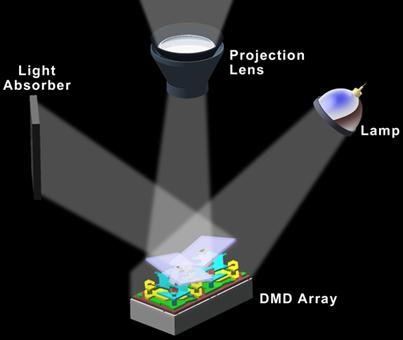
\includegraphics[width = \textwidth]{images/pixel_1.jpg}
    \label{fig:pix_left}
  \end{subfigure}
  \begin{subfigure}{0.49\textwidth}
    \centering
    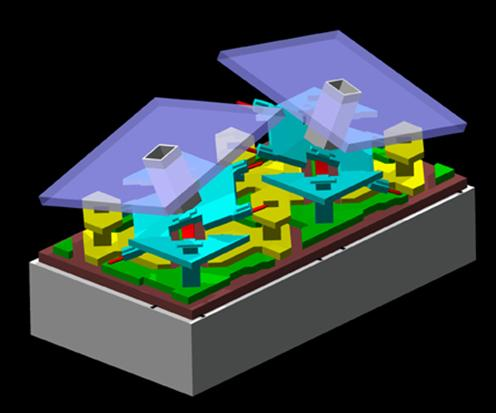
\includegraphics[width = \textwidth]{images/pixel_2.jpg}
    \label{fig:pix_right}
  \end{subfigure}
  \caption{
    \textbf{Principle of operation of a DMD in a digital projector.}
    Left, incident light can be reflected towards the projection lens (state {\em on}),
    or onto a beam dump (state {\em off}).
    Right, zoom on the pixels.
    Image adapted from \cite{JacksonDMD}.
  }
  \label{fig:combined_pixel}
\end{figure}






\section{Choosing the right DMD: Diffraction effects}

\subsection{A 1D model}

A significant distinction between liquid crystal modulators and DMDs
lies in the geometry of the pixel surface.
This difference gives rise to diffraction effects that can adversely affect
both the modulation quality and system efficiency.
The impact of these diffraction effects is highly contingent on several factors:
the wavelength of the illumination, the pixel pitch, and both the incident and outgoing angles.
Therefore, alongside selecting an appropriate anti-reflection coating,
it is crucial to ensure that the pixel pitch is compatible with the specific configuration being used.
Texas Instruments offers chips with a variety of pixel pitches $d$,
ranging approximately from $5$ to $\sim25$ \textmu m~\cite{TI}.\\


To achieve a qualitative understanding of this issue,
we consider a 1D array of pixels as illustrated in Fig.~\ref{fig:grating_geom}.
% For simplicity, we will focus on scenarios where both the incident and outgoing angles 
% are nearly perpendicular to the modulator surface, and the mirror tilt angle is minimal.
Initially, let's assume that all pixels are in the same state and are illuminated by a plane wave originating from the far field.
Under these conditions, the pixelated modulator essentially functions as a grating,
with a period $d$ that is equivalent to the pixel pitch.
It is important to underscore that these modulators possess a hardware-limited fill factor,
typically around 90\%.
This translates to an effective active pixel size of $d' < d$.\\

In general, a grating gives rise to various diffraction orders
with differing intensities
and angles $\theta_p$, as dictated by the grating equation:
$
  \text{sin}(\theta_p) = p\lambda/d = p \, \text{sin}(\theta_D),
$
where $\lambda$ is the wavelength of the light,
and $\theta_D$ is the angle of the first-order diffraction.
The intensity of the individual diffraction orders is influenced by both the size and the response of a single pixel.
Importantly, we can decouple the effects of the grating's periodicity,
which influences the angles of the diffraction orders,
from the effects of the response of a single pixel,
which shapes the envelope of the angular response.\\

\begin{figure}
  \centering
  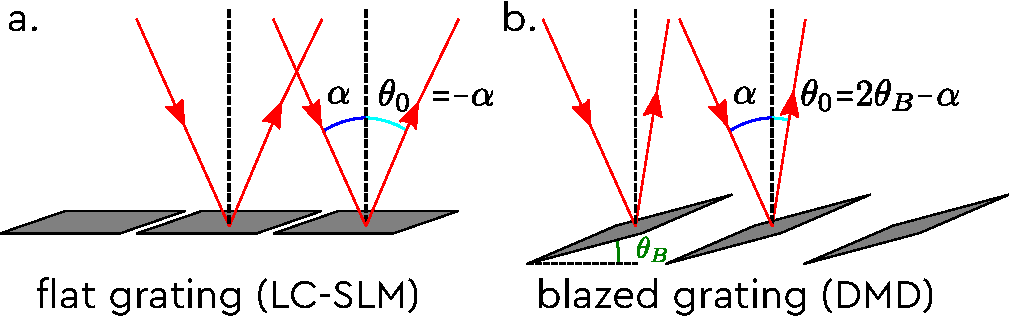
\includegraphics[width = \textwidth]{images/grating_geom.pdf}
  \caption{
    \textbf{1D grating geometry.}
    Schematic representation of the geometry of two types of modulators:
    (a) the liquid crystal modulator, equivalent to a flat grating,
    and (b) the DMD geometry, equivalent to a blazed grating.
    $\alpha$ denotes the incident angle relative to the normal of the array plane,
    $\theta_0$ refers to the angle of the zeroth diffraction order,
    and $\theta_B$ is the tilt angle of the mirrors.\\
  }
  \label{fig:grating_geom}
\end{figure}


For a case of normal incidence with an LC-SLM (Liquid Crystal Spatial Light Modulator),
we can assume that the response of a single pixel is uniform its surface.
Similarly, in the scenario of a blazed grating,
such as a DMD, a linear phase slope is present on each pixel.
This is due to the tilt angle $\theta_B$ of the mirrors.
For an arbitrarily selected incidence angle $\alpha$,
a global phase slope is introduced.
This results in a trivial shift of the angular diffraction pattern by an angle $\alpha$.
In essence, the incident angle $\alpha$ serves to shift the entire angular diffraction pattern
relative to the case of normal incidence,
while the blazed angle $\theta_B$—the tilt angle of the mirror in the DMD—
only shifts the envelope by an angle of $2\theta_B$.
Whenever the fill factor approaches 100\%,
i.e. when $d \approx d'$,
the envelope for a flat grating achieves its maximum at $\theta_0 = -\alpha$;
this corresponds to the angle of the zeroth-order diffraction,
which nears zero for all other orders.
In these specific conditions, a singular diffraction order is visually perceived, corresponding to the optimum scenario.
The addition of a blazed angle $\theta_B$ results in both
a shift in the envelope and in the position of its maximum,
now indicated by $\theta_0 = 2\theta_B - \alpha$.
In the general case,
this position may not align with a diffraction order anymore~\cite{Park2015properties}.

\begin{optional}
  Assuming the effect of the device's finite size and illumination to be negligible,
  and situating ourselves within the context of the small-angle approximation,
  we can represent the field reflected from the device
  under the influence of plane wave illumination
  across two systems as follows:


  \begin{equation}
    \begin{aligned}
      R_\text{flat}(x)   & \propto \left[\Pi\left(x/d'\right) \otimes_x \sum_k \delta(x-k d)\right]e^{-j\frac{2\pi}{\lambda}\text{sin}(\alpha) x} \\
      R_\text{blazed}(x) & \propto
      \underbrace{
        \left(
        \underbrace{\Pi\left(x/d'\right)}_\text{pixel size}
        \times
      \underbrace{e^{j\frac{2\pi}{\lambda}2\text{sin}(\theta_B-\alpha) x}}_{\substack{\text{blazed angle}                                         \\ \text{+ angle of incidence}}}
        %\text{blazed angle + angle of incidence}
        \right)
      }_\text{pixel response}
      \otimes_x
      \left[
        \underbrace{\sum_k \delta(x-k d) }_\text{periodicitiy}
        .
        \underbrace{
          e^{-j\frac{2\pi}{\lambda}\text{sin}(\alpha) kd}
        }_\text{angle of incidence}
        \right]
      \, ,
    \end{aligned}
    \label{eq:grating_response}
  \end{equation}

  with $\Pi(x)$ the rectangular function,
  representing the finite size of the pixel,
  defined as:

  \begin{equation}
    \Pi(x) =
    \begin{cases}
      1, & \text{if } -\frac{1}{2} < x < \frac{1}{2}, \\
      0, & \text{otherwise}.
    \end{cases}
  \end{equation}

  The intensity as a function of the angle in the far-field
  is given, up to a homotetic transformation,
  by the absolute value squared of

  The Fourier transform of Eq.~\ref{eq:grating_response} can be written as:






  \begin{equation}
    \begin{aligned}
      I_\text{flat}(\theta) \propto
      \sum_p \delta(\text{sin}(\theta)+\text{sin}(\alpha))
      \times
      \text{sinc}^2\left( \left[\text{sin}(\theta)+\text{sin}(\alpha)\right] \frac{\lambda}{d'}\right) \\
      I_\text{blazed}(\theta) \propto
      \underbrace{
        \sum_p \delta(\text{sin}(\theta)+\text{sin}(\alpha)-p\,\theta_D)
      }_\text{orders of diffraction}
      \times
      \underbrace{
        \text{sinc}^2\left( \left[\text{sin}(\theta)+\text{sin}(\alpha)\right] \frac{\lambda}{d'}\right)
      }_\text{envelope} \, .
    \end{aligned}
  \end{equation}

\end{optional}
A more accurate computation of the far field can be found  in ~\cite{Wang2023diffraction}.
We observe that the envelope (right hand term) is maximal for $\text{sin}(\theta_{max}) = \text{sin}(\alpha-2\theta_B)$
while the effect of the periodicity (left hand term) is maximal for $\text{sin}(\theta_p)+ \text{sin}(\alpha) = p \lambda/d$.
with $p$ an integer value.
We represent in Fig.~\ref{fig:gratings} the angular response of a flat grating and a blazed grating
for a 1D filling fraction of 95\% (correponding to a 2D filling fraction of $\approx 90$\%).
For a flat grating, only the zero-th order has a significant and comparable intensity.
For a blazed grating, in this example close to the worst case scenario,
two diffraction orders have a significant intensity,
and other orders also have a non-negligible contributions.
In the optimal scenario, where the peak of the envelope corresponds to a diffraction order,
it results in a single diffraction order carrying the majority of the energy.
This state is achieved when the conditions of the blazed grating equation are fulfilled~\cite{Casini2014on}:



\begin{equation}
  \text{sin}(2\theta_B-\alpha) + \text{sin}(\alpha)
  = 2 \,\text{sin}(\theta_B)  \,\text{sin}(\theta_B-\alpha)
  = p\frac{\lambda}{d} \, .
  \label{eq:blazed_eq}
\end{equation}



\begin{figure}
  \centering
  \begin{subfigure}{0.49\textwidth}
    \centering
    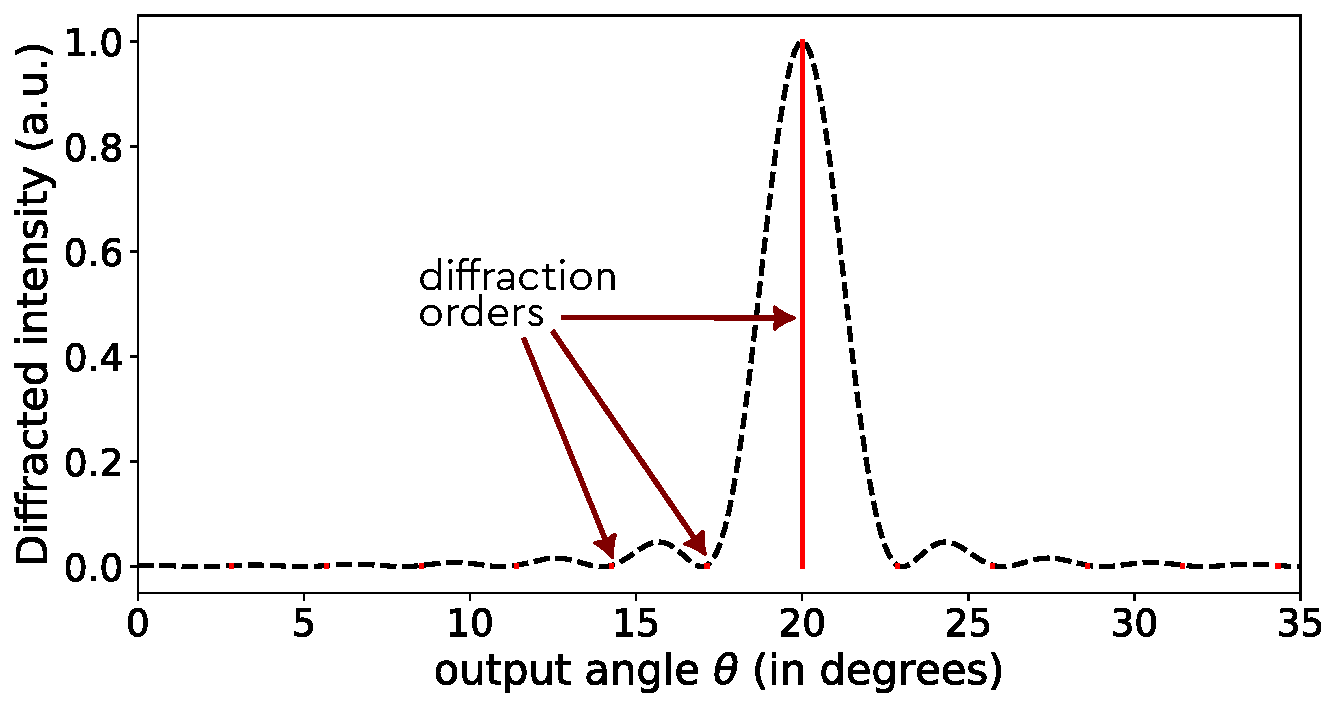
\includegraphics[width = \textwidth]{images/gratings_flat.pdf}
    \label{fig:flat_grating}
  \end{subfigure}
  \begin{subfigure}{0.49\textwidth}
    \centering
    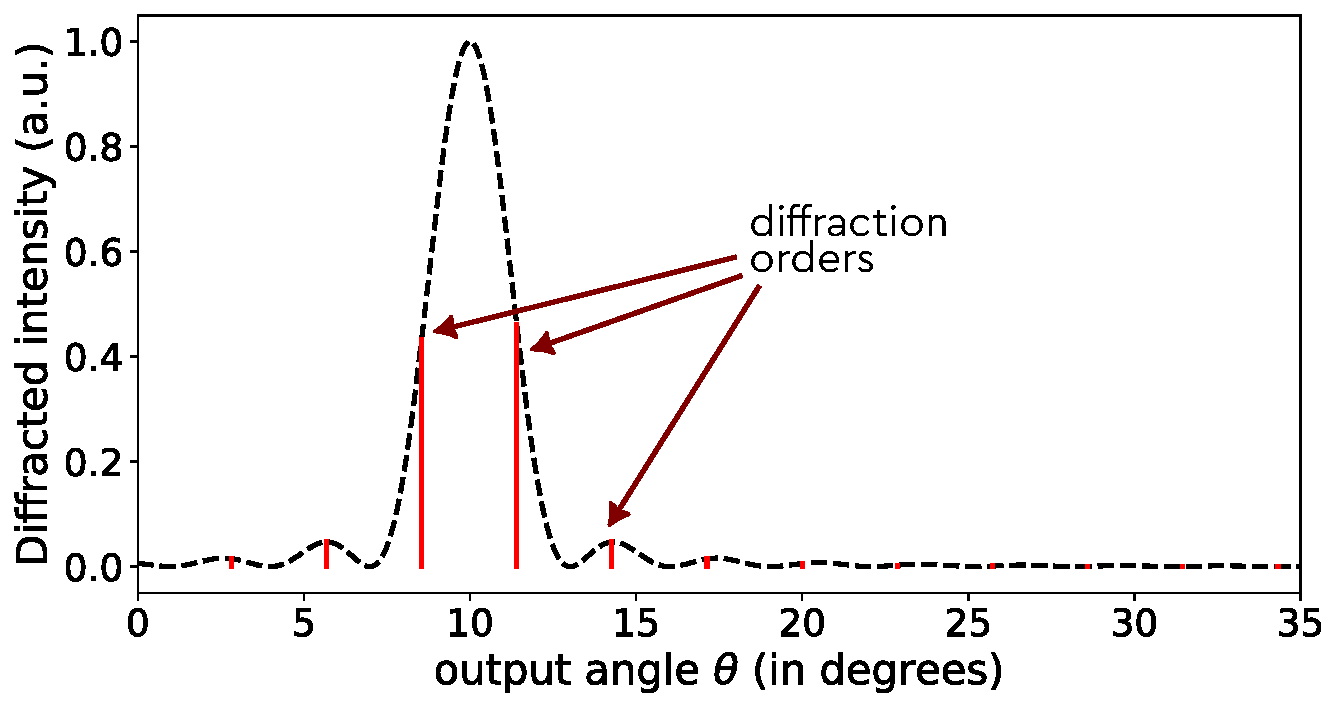
\includegraphics[width = \textwidth]{images/gratings_blazed.pdf}
    \label{fig:blazed_right}
  \end{subfigure}
  \caption{
    \textbf{Flat grating vs blazed grating.}
    Far field diffraction patterns for a 1D flat grating (left) and a 1D blazed grating (right)
    for an input angle of $\alpha = -20^\circ$,
    a filling fraction of 95\% (corresponding to a 2D filling fraction of $\approx 90$\%),
    a pixel tilt angle of $\theta_B = 5^\circ$,
    and a wavelength to pixel pitch ratio $0.05$.
    Vertical lines represent the angles of the diffraction orders
    and the black dashed curve represent the amplitude of the field.
  }
  \label{fig:gratings}
\end{figure}



% \begin{equation}
%   R_\text{flat}(x) \propto \Pi\left(x/d'\right) \otimes_x \sum_k \delta(x-k d) 
% \end{equation}

% small angle approximation
% \begin{equation}
%   R_\text{blazed}(x) \propto \left[\Pi\left(x/d'\right) \times e^{j\frac{2\pi}{\lambda}\theta_B}\right]\otimes_x \sum_k \delta(x-k d) 
% \end{equation}

\subsection{Tje 2D case}

To analyze more precisely the effect of diffraction in a DMD,
one needs to consider the 2D surface of the modulator.
We can establish a Cartesian coordinate system on the plane of the DMD,
with axes $x$ and $y$ aligned with the pixel sides
(refer to Fig.~\ref{fig:2d_geom}a).
Pixels are uniformly repeated along these axes.
However, a technical challenge arises
in that the axis of rotation of the pixels
aligns with the pixel diagonals,
resulting in a rotation by 45 degrees with respect to the $x$ and $y$ axes.
For the convenience of alignment and manipulation of the optical setup,
it is preferable to work with the incident and outgoing beams
which have the optical axis contained in the horizontal plane.
A straightforward and prevalent solution is to rotate the chip by 45 degrees
relative to the horizontal plane,
which aligns the pixel’s axis of rotation to be vertical.
This configuration is depicted in Fig.~\ref{fig:2d_geom}b.



\begin{figure}
  \centering
  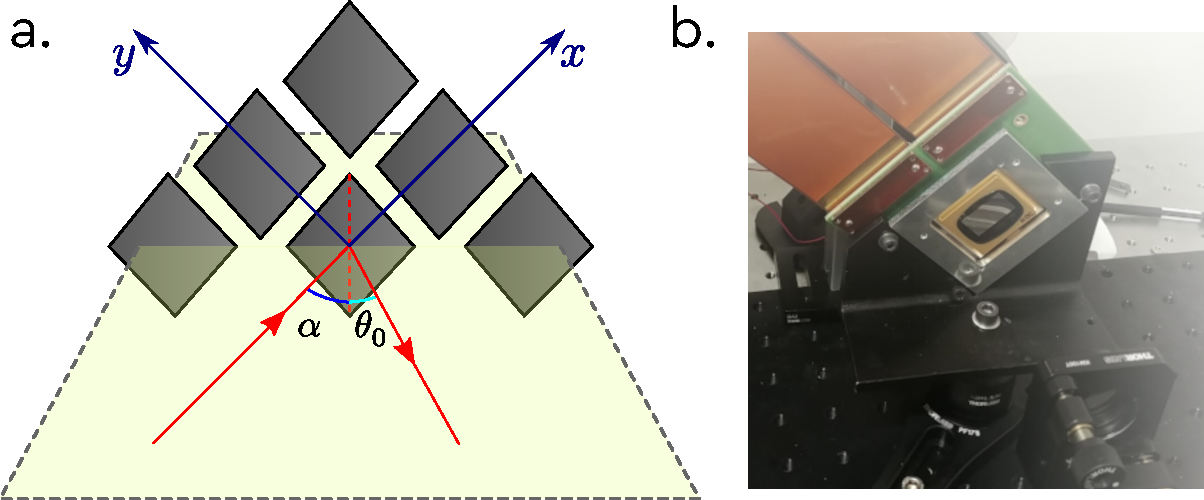
\includegraphics[width = 0.9\textwidth]{images/dmd_45.pdf}
  \caption{
    \textbf{2D grating geometry.}
    (a) Schematic representation of the geometry of the DMD.
    (b) Photograph of the DMD chip oriented so that the rotation axis of the pixels
    is aligned vertically.
  }
  \label{fig:2d_geom}
\end{figure}

The 2D array can be seen as 2 orthogonal 1D gratings in the $x$ and $y$ directions,
both having the same properties.
A more comprehensive depiction of the 2D system can be found in~\cite{Scholes2019structured}.
In order to utilize Eq.(\ref{eq:blazed_eq}),
one first needs to project
the different angles of the problem onto the incident planes
of the two 1D gratings.
This yields
$\alpha = \text{arctan}\left(\text{tan}(\alpha')/\sqrt{2}\right)$,
$\beta = \text{arctan}\left(\text{tan}(\beta')/\sqrt{2}\right)$,
and $\theta_B = \text{arctan}\left(\text{tan}(\theta_\text{DMD})/\sqrt{2}\right)$,
where $\theta_\text{DMD}$ represents the true rotation angle of the mirrors relative to the diagonal of the pixels,
and $\alpha'$ and $\beta'$ denote the incident and outgoing angles in the horizontal plane.
We can quantify how close we are to the ideal case,
i.e., when satisfying the blazed equation outlined by Eq.(\ref{eq:blazed_eq}),
by defining a {\em blazed number} $\mu$ as introduced in~\cite{WFSnet_diffraction}:



\begin{equation}
  \mu =
  \left|
  \lfloor 2 \frac{d}{\lambda}
  \left[
    \text{sin}(\alpha)  +\text{sin}(\beta)
    \right]
  \rfloor
  \mod{2} -1
  \right| \, ,
  \label{eq:blazed_number}
\end{equation}

with $\lfloor . \rfloor$ representing the integer part,
and $\mod{2}$ the modulo 2 operation.
$\mu$ is maximal and equals $1$ when the blazing equation is satisfied,
i.e. when one order of diffraction contains most of the energy,
and minimal when we are in the worst-case scenario,
i.e. when four orders of diffraction have a significant and equal intensity.\\


To demonstrate the effect, we conduct a simulation of a DMD using Python
(refer to tutorial and code in~\cite{WFSnet_diffraction})
with two pixel pitches of
$d=7.6$\textmu m and $d=10.8$\textmu m,
under a coherent excitation at $\lambda=633$nm.
Fig.~\ref{fig:mu76} shows the estimated blazed number $\mu$
as a function of the angle of incidence $\alpha'$,
along with the far field diffraction pattern for two distinct incident angles.
It should be noted that the efficiency of diffraction can be altered by adjusting
the angle of incidence, yet its impact is relatively confined
within an acceptable angular range that aligns with experimental limitations
(i.e. for angles far from $\pm 90^\circ$).
Far field patterns are centered around the maximum of the envelope
$\theta_\text{max} = 2\theta_B - \alpha$
(marked by a yellow cross).
We see that for small values of $\alpha$,
the pixel pitch of $d=10.8$\textmu m leads to a blazed number $\mu$
close $1$.
It corresponds in the far field to having one bright order of diffraction
close to the maximum of the envelope.

\begin{figure}
  \centering
  \begin{subfigure}{0.49\textwidth}
    \centering
    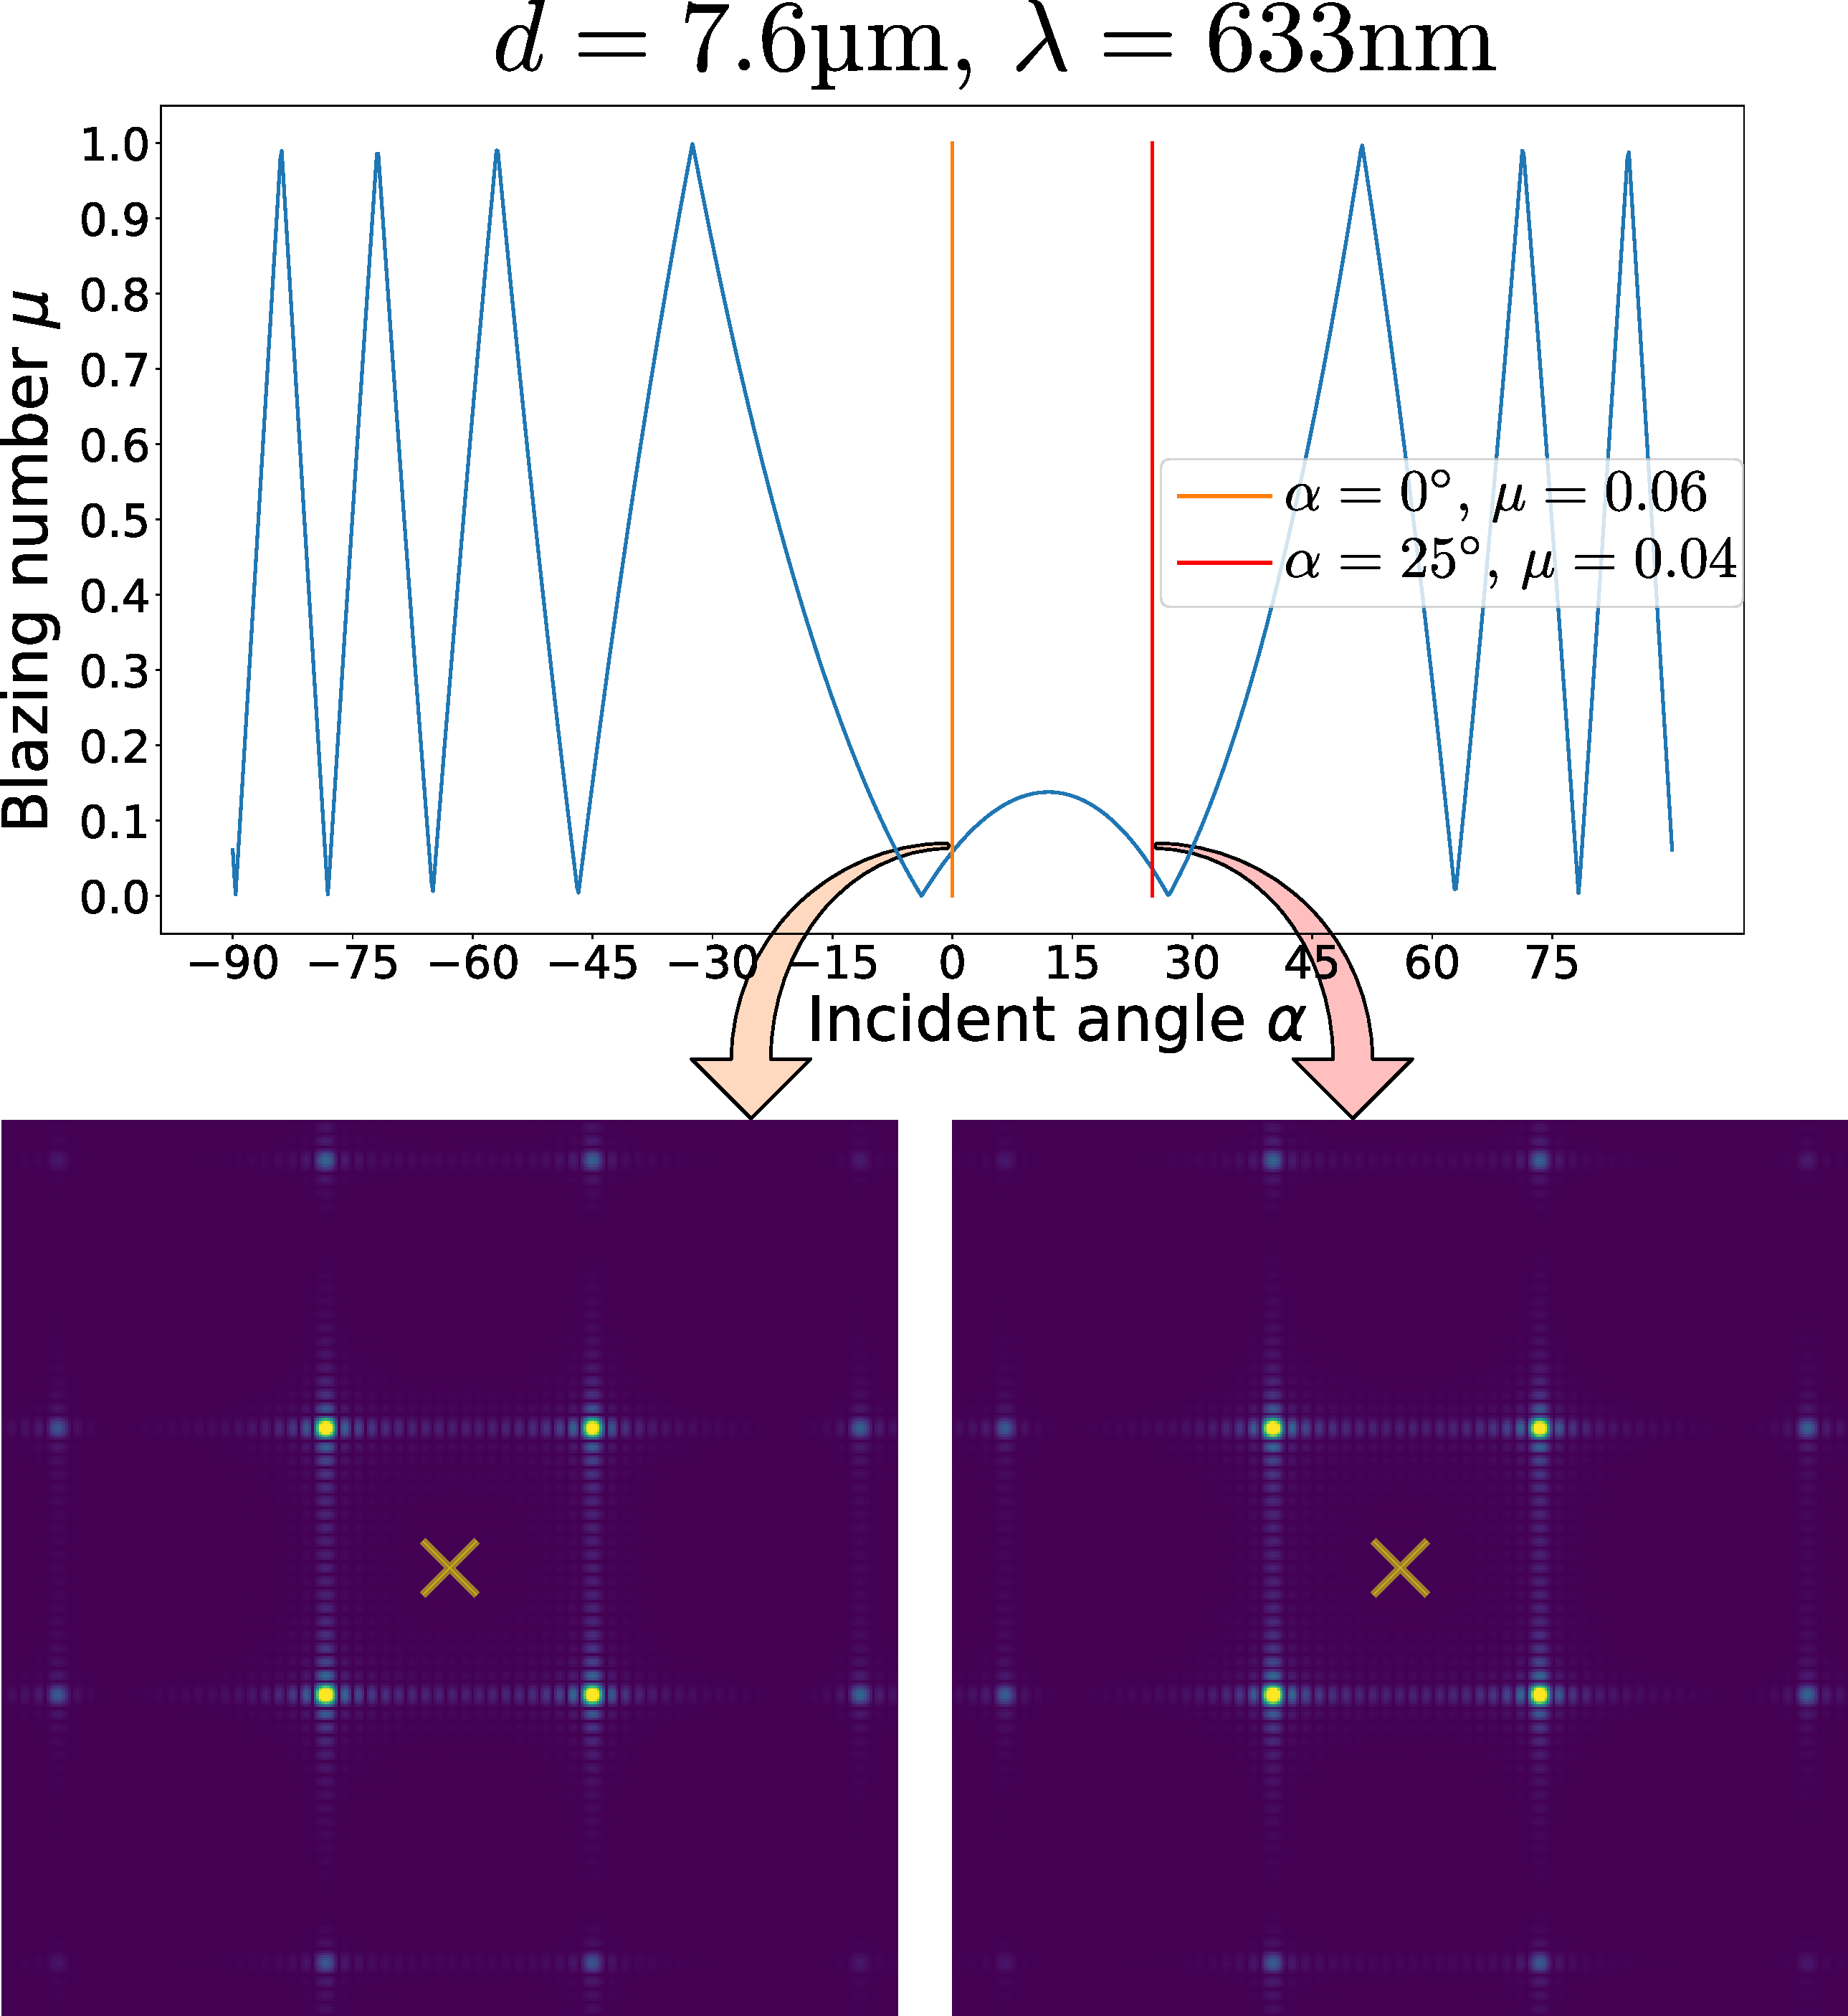
\includegraphics[width = \textwidth]{images/mu_76.pdf}
  \end{subfigure}
  \begin{subfigure}{0.49\textwidth}
    \centering
    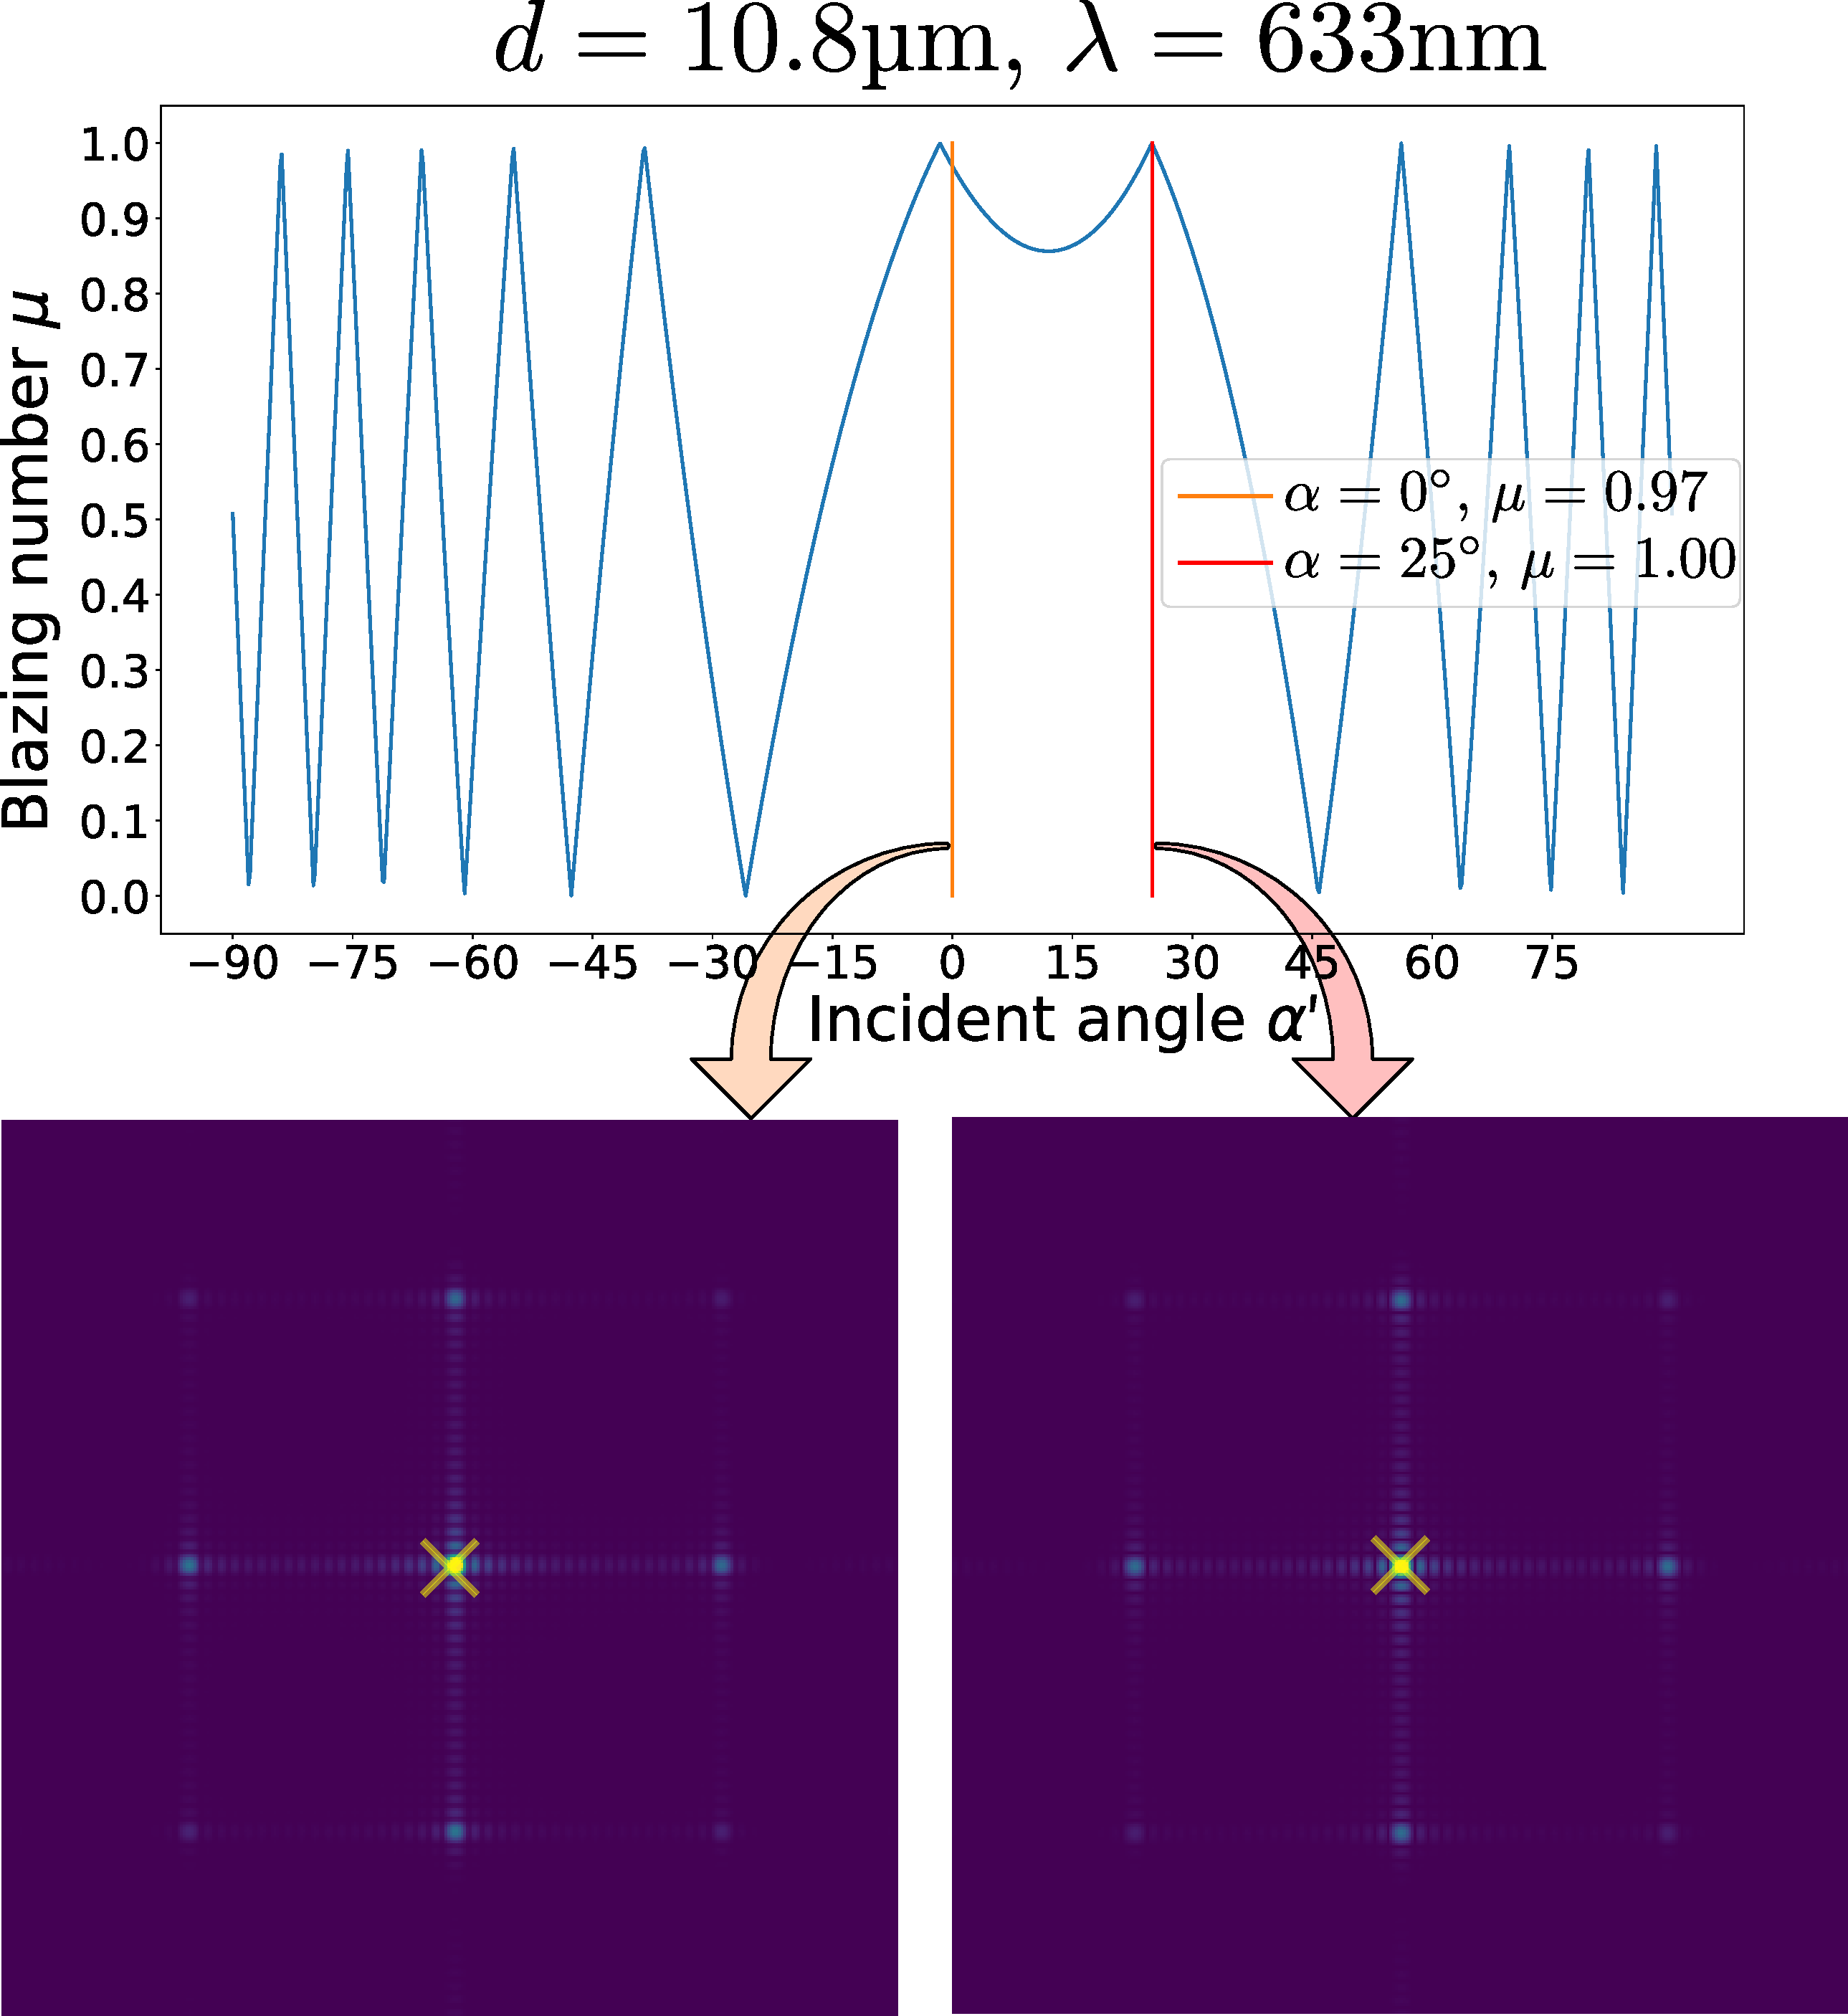
\includegraphics[width = \textwidth]{images/mu_108.pdf}
  \end{subfigure}
  \caption{
    \textbf{Blazed number and far field diffraction patterns, extreme cases.}
    Blazing number $\mu$ (Eq.(\ref{eq:blazed_number})) as a function of the incident angle $\alpha'$  (top)
    for a pixel pitch of $d=7.6$\textmu m (left)
    and $d=10.8$\textmu m (right).
    Corresponding far field diffraction pattern (bottom)
    for two incident angles $\alpha' = 0^\circ$ and $\alpha' = 25^\circ$.
    The yellow cross indicates the maximum of the envelope $\theta_\text{max} = 2\theta_B - \alpha$.
  }
  \label{fig:mu76}
\end{figure}

\subsection{Modulation cross-talk}

In practice, we place a pinhole or iris to select
one order of diffraction,
corresponding to the {\em on} state.
Having a small value for the blaze number $\mu$
not only restricts the amount of light modulation
due to the diminished diffraction efficiency,
it also influences the modulation quality by inducing cross-talk
between the two states of the DMD pixels.
Until now, we have assumed that all the pixels are in the same state.
In actual usage of the DMD,
it becomes necessary to modulate the state of each pixel individually.
When $\mu$ approaches zero, higher orders of diffraction
still possess a significant intensity,
as demonstrated in the 1D case in Fig~\ref{fig:gratings}.
One adverse implication is that pixels in the {\em off} state
may contain orders of diffraction that are not blocked by the pinhole,
and therefore, will contribute as an interference to the modulated wavefront.
While this contribution might appear weak,
it does affect the quality of the modulation
since the modulation scheme typically necessitates about half the pixels
to be in the {\em off} state for phase modulation~\cite{lee1979binary},
and even more so for elaborate modulation schemes~\cite{goorden2014superpixel,Gutierrez2024DMD}.\\



\begin{figure}
  \centering
  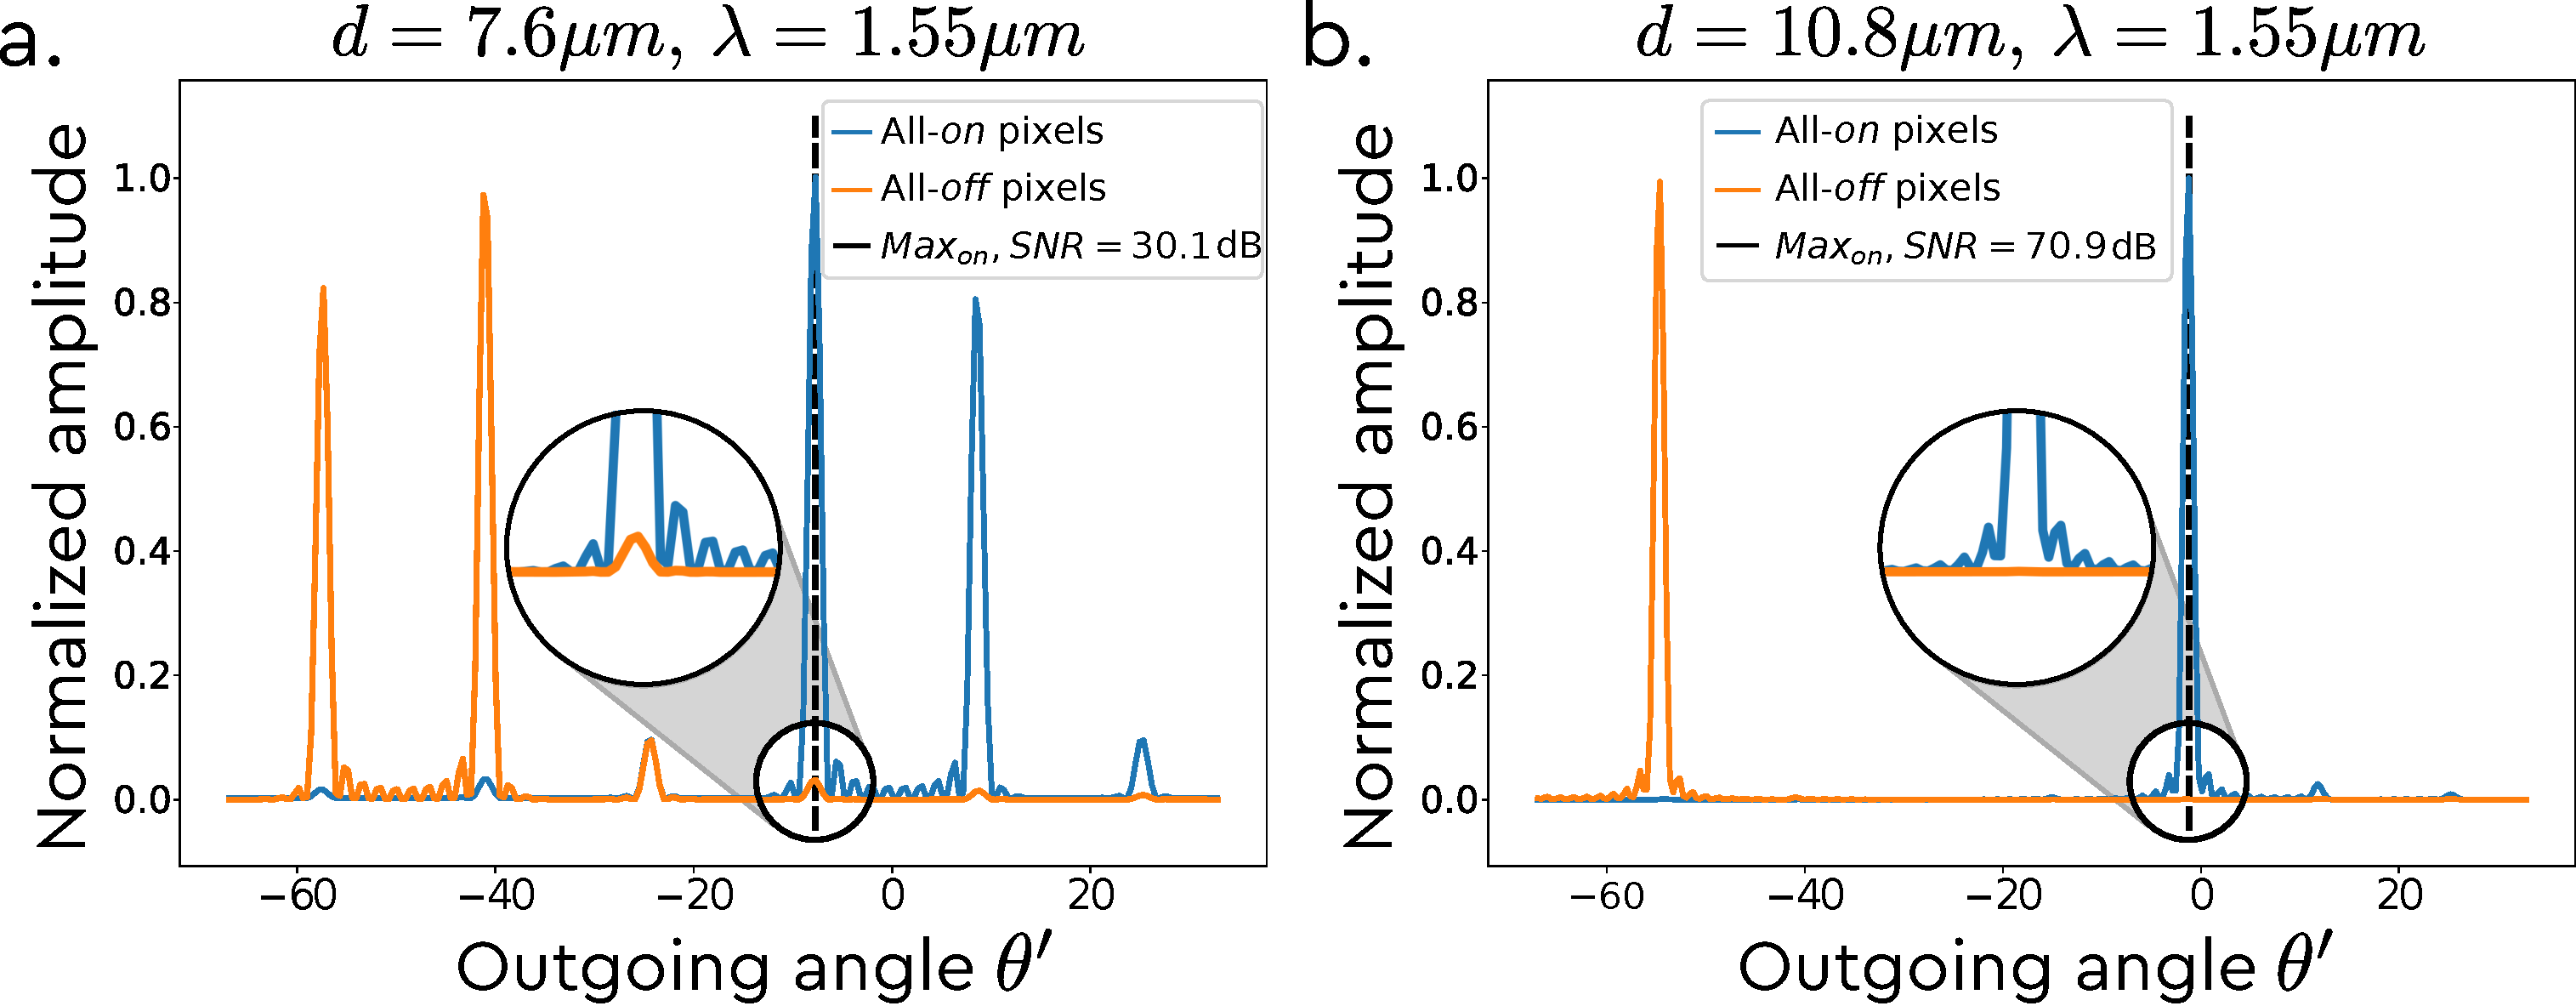
\includegraphics[width = 0.95\textwidth]{images/xtalk.pdf}
  \caption{
    \textbf{Cross-talk between {\em on} and {\em off} states.}
    We show the computed normalized amplitude of the diffraction patterns corresponding
    to all the pixels in the {\em on} state (blue)
    and {\em off} state (orange)
    for two different pixel pitches,
    $d = 7.6$\textmu m (a.)
    and $d = 10.8$\textmu m (b.)
    with the same experimental conditions.
    In the first case, $\mu$ is close to $0$,
    we observe a non-negligible contribution of the {\em off} state
    at the main diffraction order of the {\em on} state,
    thus creating unwanted cross-talk.
    In the second case, $\mu$ is close to $1$,
    the contribution of the {\em off} state is negligible.
  }
  \label{fig:xtalk}
\end{figure}
% For an incident angle $\alpha'$ 
% and a reflected angle $\beta'$ 
% in the horizontal plane,
% we can use the grating equation 
% presented in Eq.~\ref{eq:blazed_eq}

\subsection{Dispersion}


DMDs are composed of metallic small mirrors,
the response of which is minimally affected by wavelength changes.
This is particularly advantageous for broadband applications requiring amplitude modulation
and operating on a plane conjugated to the DMD's surface.
This is the case for the originally intended application of video projection.
However, for wavefront-shaping applications,
it is typically required to select a specific diffraction order
to acheive phase or complex modulation~\cite{lee1979binary,Gutierrez2024DMD}.
Under such circumstances,
the wavelength-dependency of the diffraction effect becomes important.
The blazed number, denoted by $\mu$ (according to Eq.(\ref{eq:blazed_number})),
scales inversely with the wavelength.
Fig.~\ref{fig:dispersion} shows the blazed number $\mu$
as a function of the wavelength for two pixel pitches $d=7.6$\textmu m and $d=10.8$\textmu m,
with an incident angle of $\alpha' = 20^\circ$.
Within the visible spectrum, $\mu$ fluctuates between $0$ to $1$ over a typical range of roughly 100 nm.\\



\begin{figure}[ht]
  \centering
  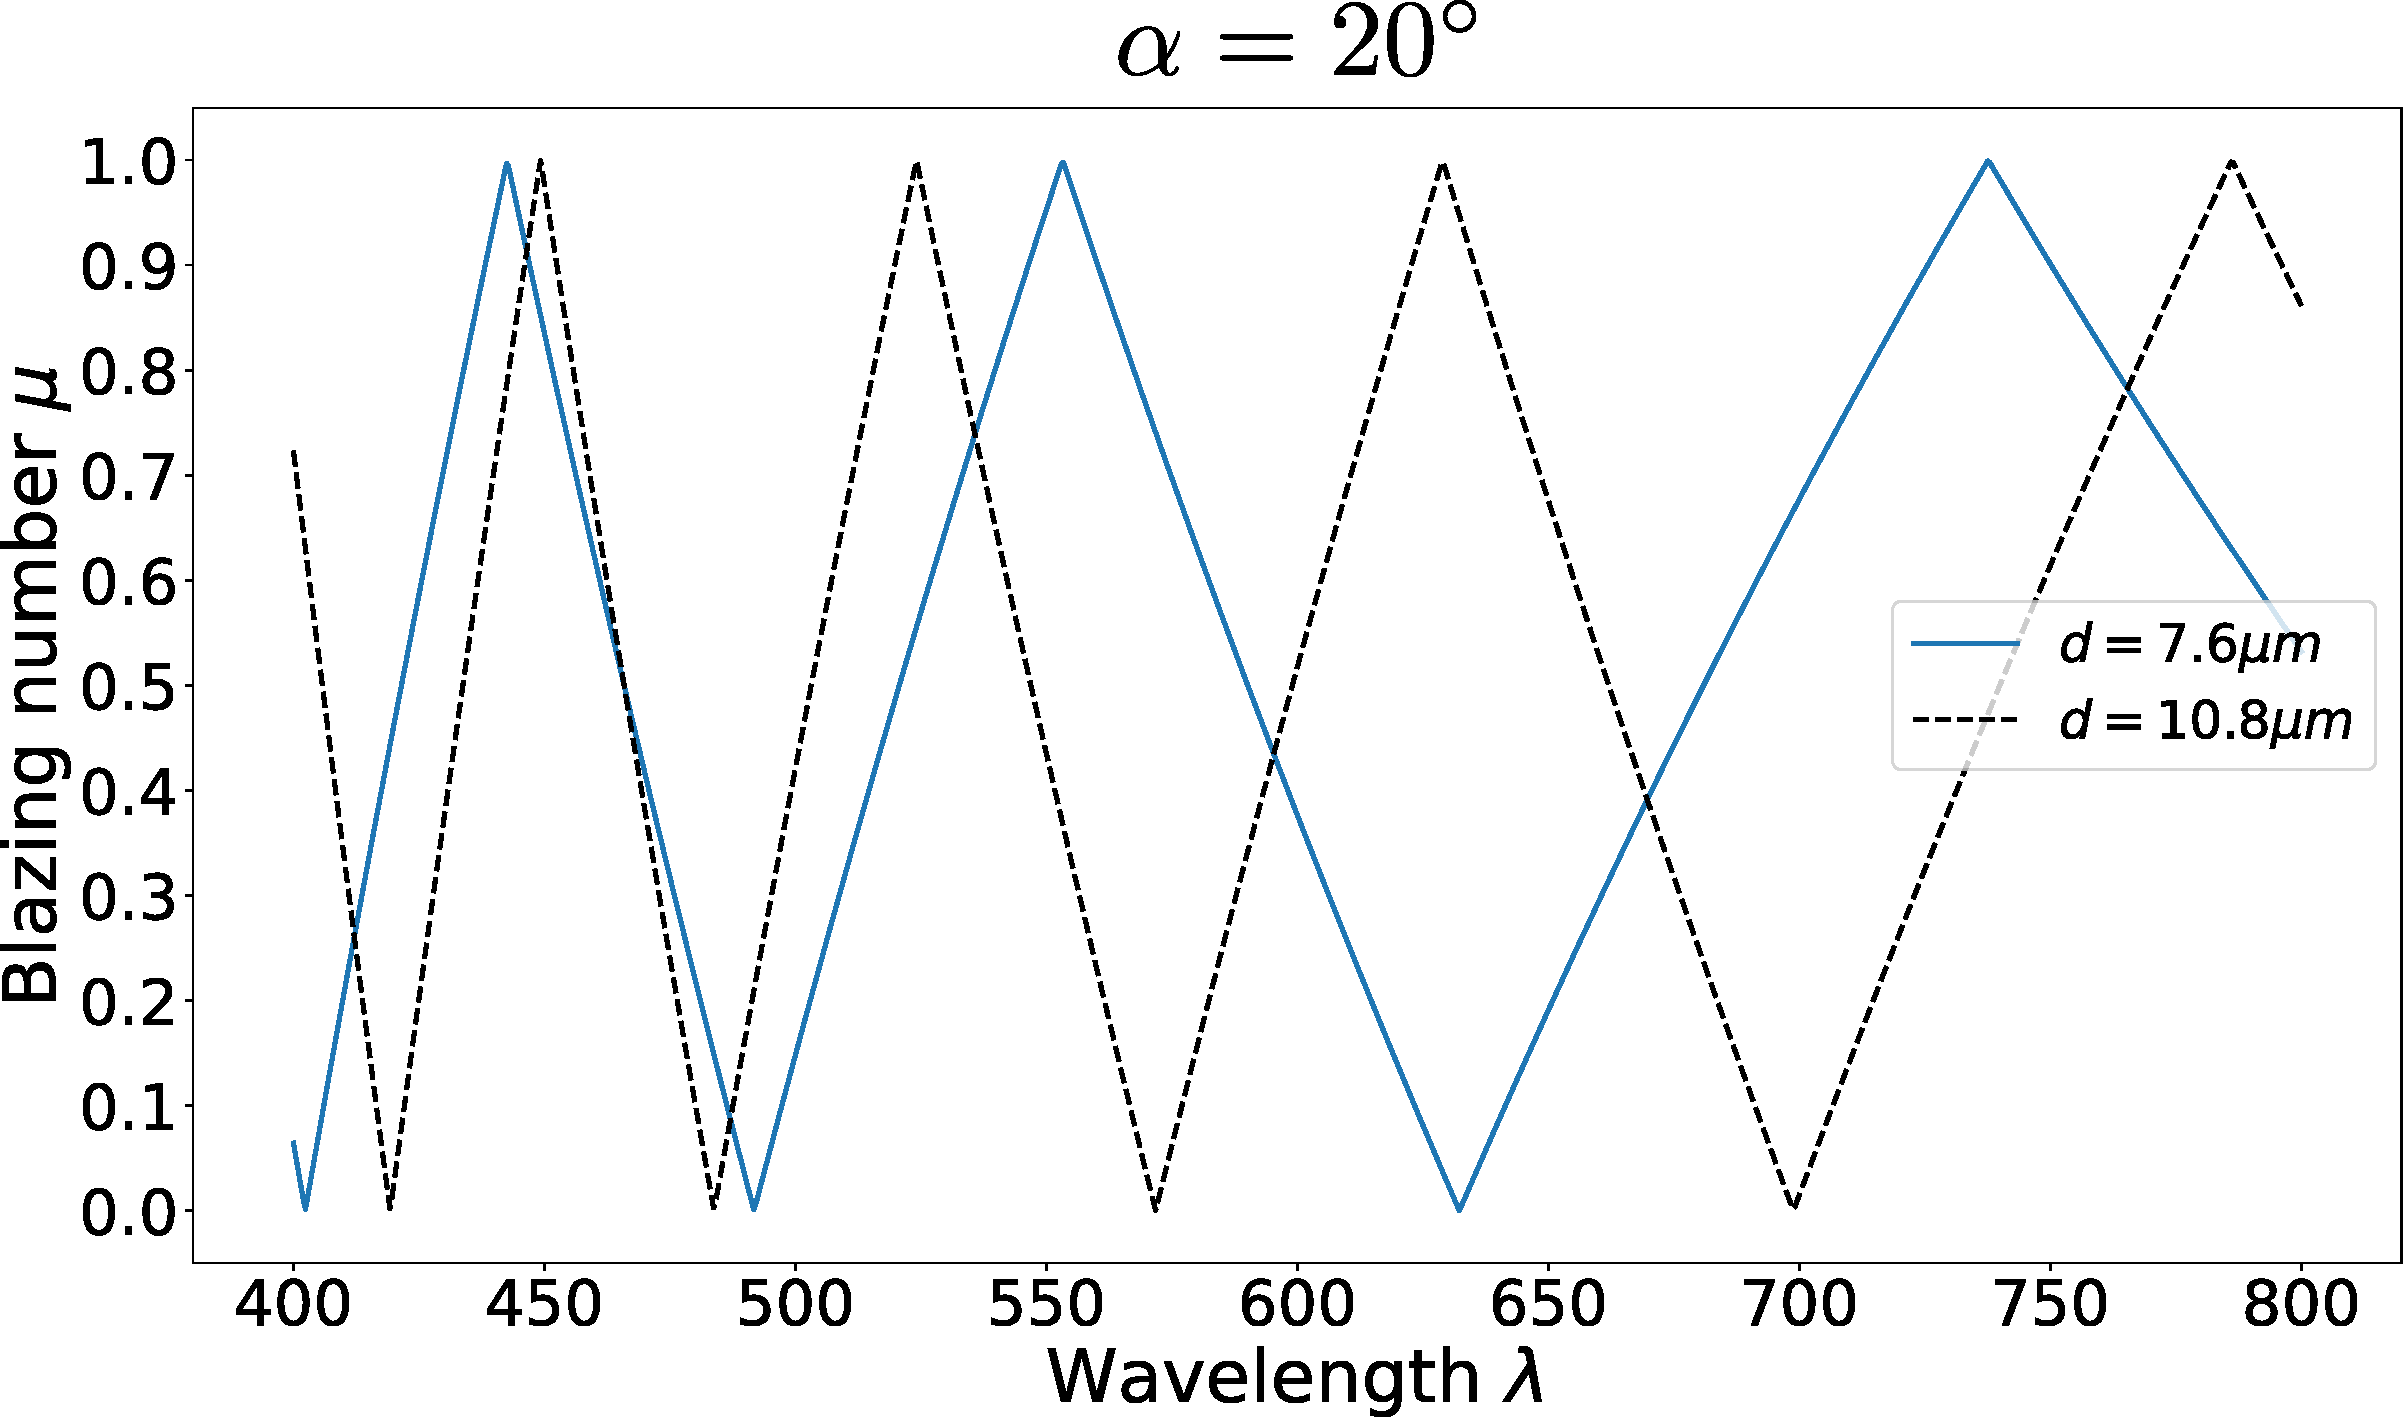
\includegraphics[width = 0.75\textwidth]{images/blazing_number_VS_wavelength.pdf}
  \caption{
    \textbf{Dispersion of the diffraction effect.}
    Blazing number $\mu$ (Eq.(\ref{eq:blazed_number})) as a function of the incident wavelength
    for an incident angle $\alpha' = 20^\circ$
    and a pixel pitch of $d=7.6$\textmu m (blue curve)
    and $d=10.8$\textmu m (dashed black curve).
  }
  \label{fig:dispersion}
\end{figure}



\begin{tldr}
  \textbf{TL;DR:}\\
  DMDs act as blazed gratings.
  For a given operation wavelength,
  we need to find the right pixel pitch
  to have a good modulation quality
  and diffraction efficiency.
  It can be done by estimating the \textit{blazed number} $\mu$ introduced in eq.~(\ref{eq:blazed_number})
  or directly using our custom online tool~\cite{popoffDMDDiffractionTool}.
\end{tldr}


\subsection{Python code example}

We provide in the paper repository~\cite{github} a Python code
to simulate the diffraction effect of a DMD
by computing the far field pattern for a set of realistic parameters.
It provides a simple way to estimate the blazed number $\mu$ introduced in eq.~(\ref{eq:blazed_number})
to assess the quality of the modulation at the desired wavelength
for a given pixel pitch.
We also propose an online tool accessible at
\url{https://www.wavefrontshaping.net/post/id/49}.




% Let's consider first a 1D toy model to have a qualitative understanding of the problem.


% Liquid crystal pixels are flat and aligned with the array surface. 
% The periodicity of the pixels makes the device behave as a flat grating. 
% Thus, the reflection angle is the opposite of the incident one compared to the normal of the array plane. 
% That implies that the path coming from each element of the device has the same optical path length 
% (see Fig.~\ref{fig:reflection} left). 


% In a DMD, the modulation is achieved by setting each pixel to one of two states, 
% corrsponding to angles $\pm \theta$ with respect to the the normal of the array plane. 
% It thus acts as a blazed grating.
% Two consecutive pixels, or elements, now give rise to a phase difference 
% between two parallel rays reflected of neighboring pixels (see Fig.~\ref{fig:reflection} right). 
% In the Fourier plane, where we commonly select the zero-th order, all the diffraction orders are shifted compared to the optical axis within the same envelope. In the worst scenario, we can end up with four diffraction orders with approximately the same intensity, each significantly shifted compared to the optical axis. An example is shown in Figure 6. This is almost exactly what I had the first time I set up my DMD while I expected something like in Figure 5.

% Another way of seeing this effect is to consider that the diffraction orders (satisfying the grating equation) do not match anymore the angle of the reflected beam.

% We first use a 1D model to evaluate the effect of the tilt angle on the diffraction pattern. We then use simple numerical calculations to estimate the profile of the diffraction pattern. The full Python code used in this post is available as an IPython Notebook on my GitHub account: blazing_angle_DMD.ipynb.



%%%%%%%%%%%%%%%%%%%%%%%%%%%%%%%%%%%%%%%%%%%%%%%%%%%%%%%%%%%%%%
%%%%%%%%%%%%%%%%%%%%%%%%%%%%%%%%%%%%%%%%%%%%%%%%%%%%%%%%%%%%%%
%%%%%%%%%%%%%%%%%%%%%% ABERRATIONS %%%%%%%%%%%%%%%%%%%%%%%%%%%
%%%%%%%%%%%%%%%%%%%%%%%%%%%%%%%%%%%%%%%%%%%%%%%%%%%%%%%%%%%%%%
%%%%%%%%%%%%%%%%%%%%%%%%%%%%%%%%%%%%%%%%%%%%%%%%%%%%%%%%%%%%%%


\section{Characterizing aberration effects}

\subsection{Presentation of the problem}

While only capable of providing hardware binary amplitude modulation,
DMDs serve as a potent tool for wavefront shaping and sensing.
These applications  critically require characterization and correction of aberrations
caused by the non-flatness of the DMD surface.
For LC-SLMs, the manufacturer typically characterizes the surface's inhomogeneities within the plane of the modulator and
provides a spatial phase profile of the introduced aberrations based on the operational wavelength.
It is noteworthy that when utilized for intensity modulation on a plane conjugated to the DMD plane,
as it is done in digital projectors,
the system becomes insensitive to the aberrations caused by the DMD surface.
Consequently, these effects are commonly overlooked and rarely documented in the information provided by the manufacturers.
Nonetheless, they are non-negligible, with deviations from a flat surface
that typically spans several wavelengths~\cite{Brown2021multicolor}.\\



\subsection{Finding the correction pattern}

In the literature, various methods have been proposed to characterize
the phase pattern of the DMD aberrations in the plane of the modulator.
Typically, this involves using a model for the aberrations,
tweaking the parameters to align with the measurements~\cite{Matthes2019Optical,Scholes2019structured, Brown2021multicolor}.
An alternative approach entails direct measurement of the distorted wavefront,
either employing a wavefront sensor such as a Shack-Hartmann~\cite{Lee2023compensation},
or via interferometry.
While such methods yield accurate results,
they necessitate adaptation to the particular
setup conditions,
and frequently require supplementary optical components,
meticulous alignment,
and custom software.
Furthermore, they also demand
a meticulously calibrated and stable setup.
In this section, we introduce a straightforward method to characterize the aberrations using a lens and a camera.
This technique can be employed for any system that offers phase modulation,
such as LC-SLMs or deformable mirrors. \\



\begin{figure}
  \centering
  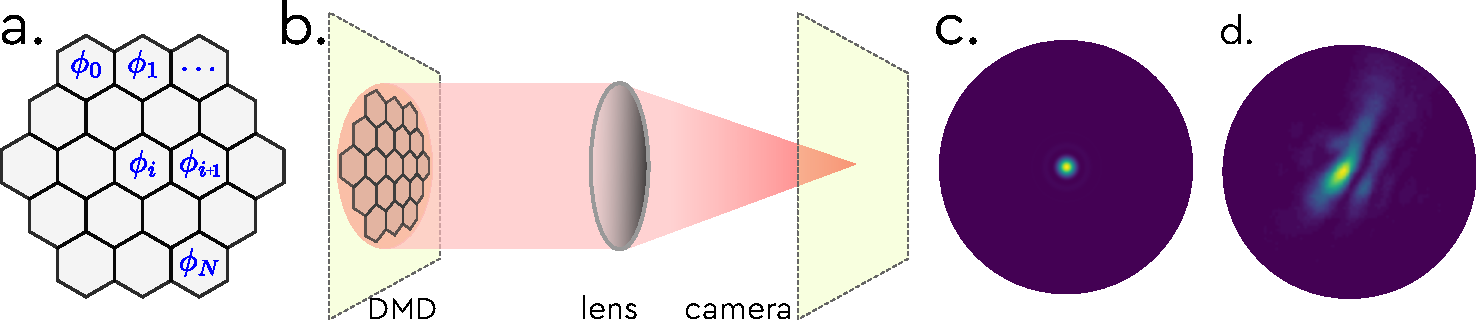
\includegraphics[width = 0.95\textwidth]{images/DMD_abberations_setup.pdf}
  \caption{
    \textbf{Setup for aberration correction.}
    (a) A schematic representation of the DMD array divided into macropixels,
    of which the phase can be controlled.
    The precise shape of the macropixels and the area controlled are not crucial for the characterization of aberrations to be effective,
    provided that the spatial sampling is sufficient to capture the highest spatial frequencies of the aberrations.
    (b) A schematic representation of the setup employed to characterize the aberrations.
    A camera is used to image the far field on the DMD surface using a lens.
    (c) shows the ideal intensity pattern corresponding to the numerical aperture of the illumination setup,
    i.e. its theoretical ideal point spread function.
    (d) show the actual recorded intensity pattern corresponding to a distorted point spread function due to the DMD aberrations.
  }
  \label{fig:dmd_aberr_setup}
\end{figure}


We assume the DMD is configured to deliver phase modulation~\cite{lee1979binary,Gutierrez2024DMD}.
This implies that the modulator can be divided into $N$ sections,
which we designate as {\em macropixels},
where the phase can be controlled independently.
We use a lens and a camera in its Fourier plane,
illuminating the modulator with a collimated beam
that extends over the entire area of the modulator intended for use.
In scenarios where there are minimal or no aberrations,
the intensity pattern observed would mimic the PSF of the lens,
such as an Airy disk depicted in Fig.~\ref{fig:dmd_aberr_setup}.c.
However, in practice, we encounter a substantially distorted pattern,
like the one represented in Fig.~\ref{fig:dmd_aberr_setup}.d.
A more detailed depiction of the setup for aberration characterization,
in the context of a wavefront shaping application in complex media is presented in Fig.~\ref{fig:dmd_aberr_setup2}.a.
In the case where the medium is a multimode fiber,
one could leverage the reflection from the input surface
to directly visualize the intensity pattern of the input plane,
as shown in Fig.~\ref{fig:dmd_aberr_setup2}.b.\\

\begin{figure}
  \centering
  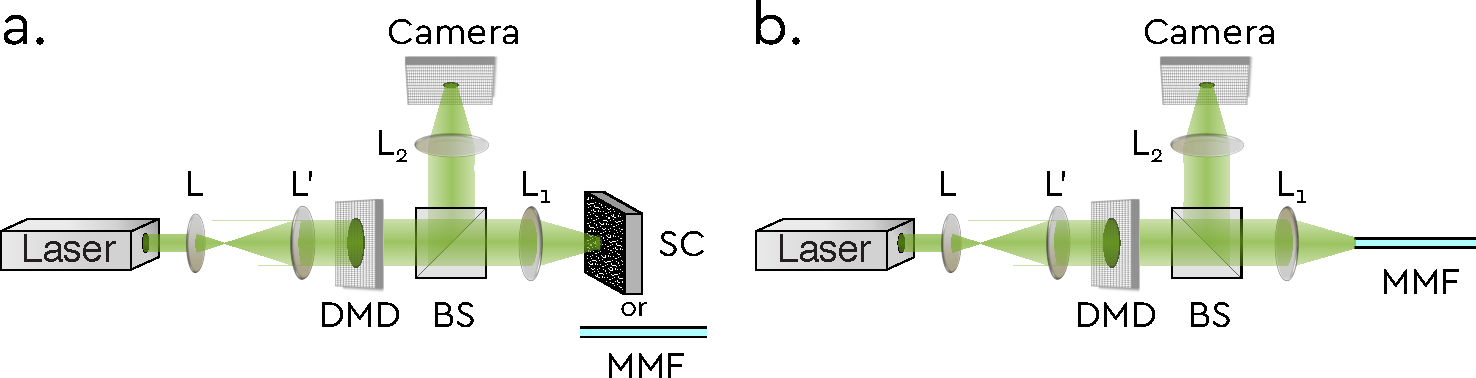
\includegraphics[width = 0.95\textwidth]{images/aberr_setup.pdf}
  \caption{
    \textbf{Detailed aberration characterization setup.}
    (a) A laser beam is expanded and collimated using a telescope (lenses L and L').
    The DMD is represented in transmission for simplicity.
    Light reflected from the DMD is focused by a lens L$_\text{1}$
    onto the complex medium to study, namely a scattering medium (SC)
    or a multimode fiber (MMF).
    A beamsplitter is used to image the far field of the DMD onto a camera
    using a lens (L$_\text{2}$).
    The intensity pattern, up to a homotetic transformation,
    represent the input excitation on the medium
    which also corresponds to the PSF of the illumination setup.
    (b) In the case of a multimode fiber,
    one can take advantage of the reflection of the input facet
    to directly image the intensity pattern of the input plane.
  }
  \label{fig:dmd_aberr_setup2}
\end{figure}

We hypothesize that the aberrations brought about by the DMD are smooth,
and can be depicted by a phase pattern $\phi^\text{aber}$ in the plane of the DMD array.
This could be feasibly approximated by a finite number of Zernike polynomials
$Z_n(r,\theta)$~\cite{Zernike1934beugungstheorie}, as follows:



\begin{equation}
  \phi^\text{aberr}(r,\theta) \approx \sum_{n=0}^N a_n Z_n(r,\theta) \, .
\end{equation}

The goal is to find and display the phase value
$\phi_i^\text{corr}$ on each macropixel $i$ that best compensates for the aberrations,
i.e. $\phi_i^\text{corr} = -\phi^\text{aber}(r_i,\theta_i)$.
We create this pattern in the basis of Zernike polynomials

\begin{equation}
  \phi_i^\text{corr} = \sum_{n=0}^N a'_n Z_n(r,\theta) \, ,
\end{equation}

the best correction if obtained for


\begin{equation}
  a'_n = -a_n \,\, \forall n \in [0..N]\, .
\end{equation}

\begin{figure}
  \centering
  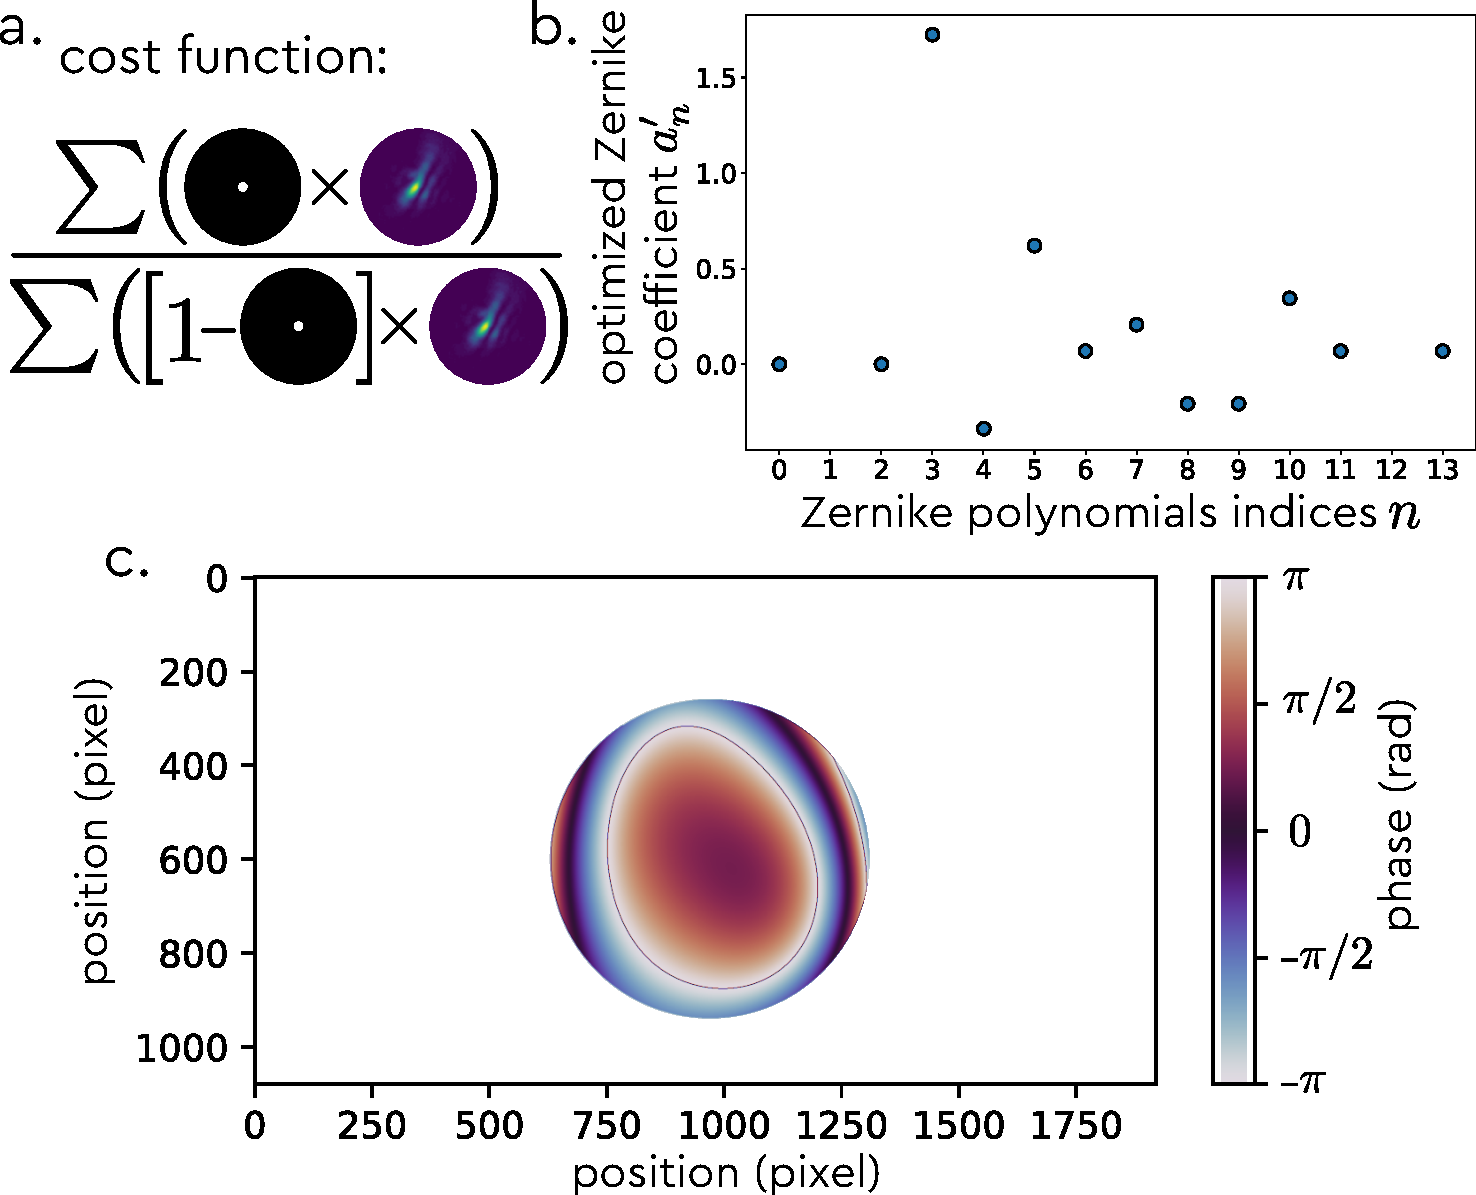
\includegraphics[width = 0.95\textwidth]{images/Zernike_1.pdf}
  \caption{
    \textbf{Correction phase map.}
    (a) Schematic representation of the function we want to optimize.
    We both want to maximize the intensity of the main lobe of the point spread function
    and minimize its side lobes.
    (b) Values of the experimentally obtained optimal coefficients in the Zernike polynomials basis.
    (c) Resulting optimal phase pattern in the chosen illumination area.
  }
  \label{fig:phase_corr}
\end{figure}

We perform a sequential optimization of parameters $a_n$
to maximize a specific function designed
to be maximal for the ideal correction of optical aberrations.
We first  generate a mask, represented by a disk,
centered around the point of maximum intensity of the original image (refer to Fig.~\ref{fig:dmd_aberr_setup}.d)
with a radius equivalent to a single speckle grain.
The exact size of this radius for a successful optimization is not critical
and can be determined by approximating the dimensions of the ideal point spread function,
expressed as $r_0 \approx M \frac{\lambda}{2 NA}$,
where $NA$ is the numerical aperture of the optical system and $M$ refers to its magnification.
For a given output intensity pattern, we compute an element-wise product between this image
and the created mask, followed by a summation.
This calculated sum is then divided by an analogous product, but with the complementary mask substituted in place of the original
in order to minimize the side lobes of the point spread function.
We set initial parameter values as $a'_n = 0\,\, \forall n \in [0..N]$.
For each parameter, we test different values of $a'_n$,
construct the phases for every micropixel according to
$\phi_i^\text{corr} = \sum_{n=0}^N a'_n Z_n(r_i,\theta_i)$,
record the resulting intensity profile,
and evaluate the corresponding cost function.
For each parameter, the value that results in the maximum output is retained.
To mitigate potential noise or instability, this complete process is reiterated $3$ times for each parameter.\\


To estimate the quality of the correction,
we compute the Strehl ratio of the point spread function.
It is defined as the maximum of the measured PSF divided
by the maximum of the ideal one.
This optimal PSF is
the  squared modulus of the Fourier transform of a circular aperture~\cite{airy1835diffraction}:

\begin{equation}
  PSF_\text{ideal} \propto
  \left[
    J_1\left(k a \frac{R}{\sqrt{R^2+f^2}}\right)
    \right]^2 \, ,
\end{equation}

with $J_1$ the Bessel function of the first kind of order $1$,
$k = 2\pi/\lambda$ the wavenumber,
$a$ the radius of the aperture,
$R$ the radial coordinate in the Fourier plane,
and $f$ the focal length of the lens.\\


As an illustration, we conduct an optimization procedure using 11 Zernike polynomials.
We use a V-9501 Vialux DMD with a DLP9500 TI chip
of resolution 1920 by 1200 pixels and a pixel pitch of 10.8 \textmu m.
The optimization is performed on a disk of radius $340$ pixels,
The illumination is done using an expanded laser beam at 633 nm,
corresponding to the aperture of our optical setup.
We exclude the first three Zernike polynomials in the optimization process,
starting from the radial degree $2$.
Indeed, the initial one, known as the piston, does not influence the PSF quality.
The subsequent ones, the tip and the tilt, cause the PSF to shift.
Our procedure relies on optimizing the maximum of the PSF, wherever that is,
rendering us indifferent to these two parameters.
After optimization,
it is possible to generate the correction pattern using a selected number of Zernike polynomials
in order to investigate their impact on the PSF quality.
We see here that using about 10 Zernike polynomials is sufficient to obtain a Strehl ratio $>0.99$.
Fig.~\ref{fig:zernike} demonstrates the Strehl ratio and the intensity profiles of the PSF
for different counts of the utilized Zernike polynomials.
It is important to note that we do not use the full surface of the DMD.
Using a larger area may lead to stronger deformations of the PSF,
requiring a larger number of Zernike polynomials to be corrected accurately.
The experimental data, in addition to the Python code used to generate the figures, can be accessed in the dedicated repository~\cite{github}.\\





\begin{figure}
  \centering
  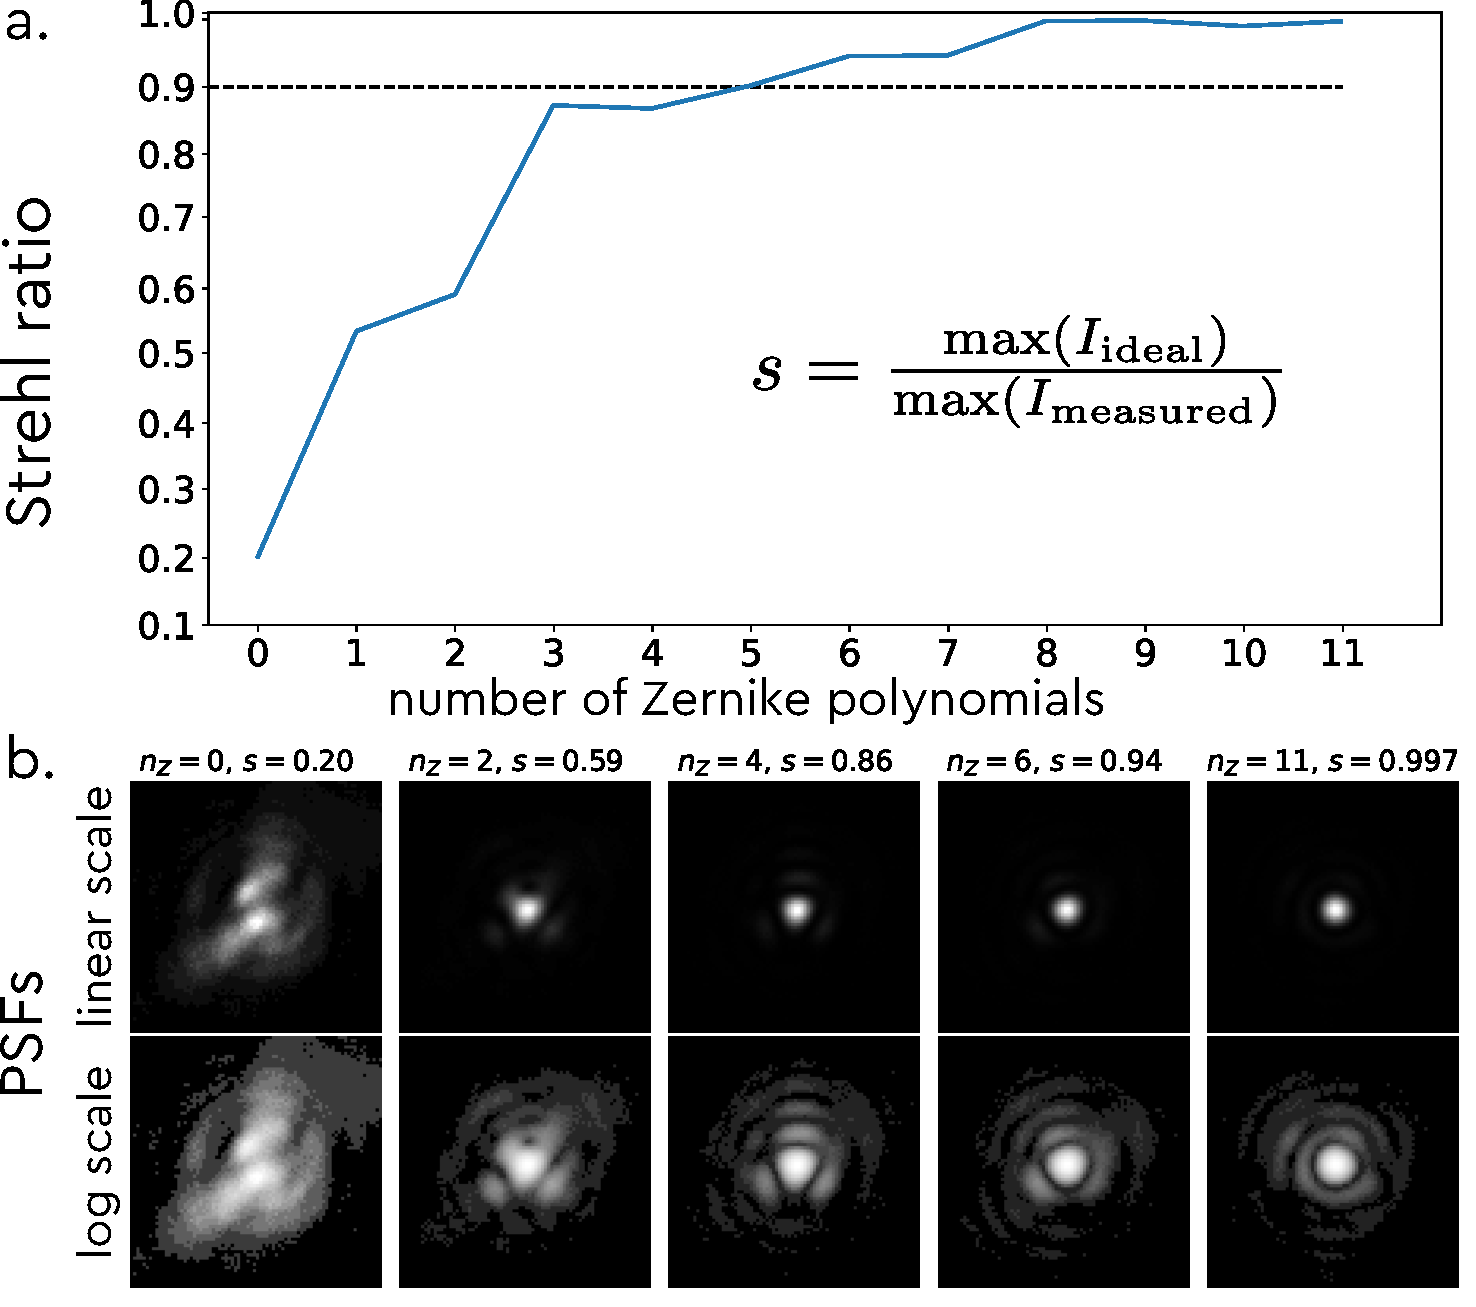
\includegraphics[width = 0.95\textwidth]{images/Zernike_2.pdf}
  \caption{
    \textbf{Effect of Zernike polynomials on the optimization of the PSF.}
    (a) Strehl ratio of the point spread function as a function of the number of Zernike polynomials used
    for the compensation of the aberrations.
    (b) Intensity profile of the point spread function for different number of Zernike polynomials
    in linear and logarithmic scale.
    To generate this data, we take the final solution of the optimization experimental procedure,
    i.e. the optimal coefficients $a'_n$,
    and generate the corrected PSF with an increasing number of Zernike polynomials.
  }
  \label{fig:zernike}
\end{figure}


\subsection{Python code example}

We provide in the paper repository~\cite{github} a Python code example
to simulate the effect of aberration on a DMD
and then perform a sequential optimization as previously proposed
to learn the characterize pattern.
We make use of the !aotools! package~\cite{Townson2019aotools} for generating Zernike polynomials.

% In this section, we provide Python code snippets for performing aberration correction.
% We presuppose that phase modulation can be controlled using a function,
% !display_phase_mask(phase_pattern)!, to display a desired phase pattern
% with real values between $0$ and $2\pi$.
% It is important to note that phase modulation utilizing a DMD demands an appropriate setup
% and process. Although not detailed here,
% this is elaborated upon in the referenced tutorial~\cite{Gutierrez2024DMD}.
% Additionally, we assume the existence of a function, !get_camera_image()!,
% which returns the intensity pattern as measured by the camera.



\begin{tldr}
  \textbf{TL;DR:}\\
  DMDs are not flat and can introduce aberrations;
  these are typically much stronger than those commonly observed with liquid crystal SLMs.
  This can be counteracted in situ using a standard setup and a straightforward optimization procedure
  to maximize the intensity at the central position of the point spread function.
\end{tldr}

%%%%%%%%%%%%%%%%%%%%%%%%%%%%%%%%%%%%%%%%%%%%%%%%%%%%%%%%%%%%%
%%%%%%%%%%%%%%%%%%%% 4. STABILITY %%%%%%%%%%%%%%%%%%%%%%%%%%%
%%%%%%%%%%%%%%%%%%%%%%%%%%%%%%%%%%%%%%%%%%%%%%%%%%%%%%%%%%%%%

\section{Mechanical and thermal stability}

Unlike the original purpose of the DMD, i.e. amplitude modulation for video projectors,
typical scientific applications require a high stability of the generated wavefront.
This is particularly true for applications in complex media,
such as strongly scattering media or multimode fiber,
where a small change in the phase front can lead to a large change in the output intensity profile.
While LC-SLMs design has been improved and adapted to scientific applications
over the last decades,
DMD are still relatively new tools for wavefront shaping and sensing
and are prone to instabilities that need to be addressed by the user.
In this section, we present the effect of mechanical and thermal instabilities
and how to limit their impact on the wavefront quality with simple solutions.\\


\subsection{Mechanical stability}


Most DMD kits consist of two primary components,
the chip itself and the electronic board that controls it.
This could be the standard electronics board typically used for video projectors,
as seen in TI evaluation kits,
or an FPGA specifically designed for rapid scientific usage,
as offered by Vialux~\cite{vialux} for instance.
Integral to these electronics is a fan designed to cool both the chip and the electronic board.
However, due to the use of a rigid flat cable for connection between the chip and the electronics board,
these parts are not mechanically independent.
As such, vibrations originating from the board are partially transmitted to the chip,
resulting in minute rotations of the mirror surface.
Although this perturbation is inconsequential for video projection,
they can have significant impacts on applications involving complex media
given their high sensitivity to phase front variations.\\


Due to its high sensitivity in complex media,
it is convenient to characterize this effect
directly on the system's response,
rather than constructing a distinct setup to analyze the wavefront itself.
An example of such a setup is demonstrated in Fig.~\ref{fig:MMF_ref},
although a similar approach can be employed with a scattering medium.
We enlarge a laser beam onto the DMD and transmit the incoming light through a multimode fiber.
Additional elements are required in the setup to fulfill the requirement for complex modulation~\cite{Gutierrez2024DMD}.
For the sake of clarity, we present a simplified version of the setup where those elements are not present.
The output from the fiber is then made to interfere with a reference arm
in an off-axis configuration~\cite{Cuche2000spatial},
allowing us to detect changes in the output complex field
by recording the interference pattern using a camera.\\




\begin{figure}[ht]
  \centering
  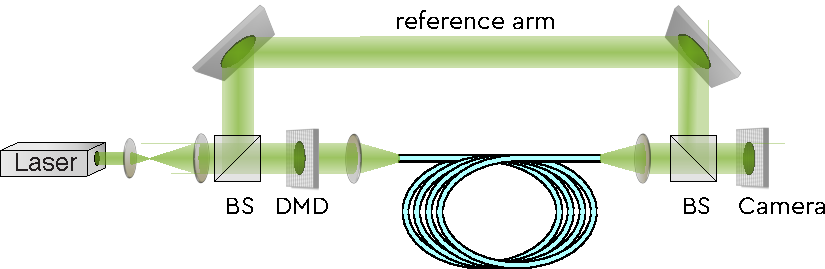
\includegraphics[width = 0.95\textwidth]{images/MMF_ref.pdf}
  \caption{
    \textbf{Measuring stability at the output of a multimode fiber.}
    Schematic representation of the setup used to measure the phase fluctuations
    through a multimode fiber.
    An equivalent setup can be used with a scattering medium.
  }
  \label{fig:MMF_ref}
\end{figure}

In the supplementary materials~\cite{SI}, we present an animation illustrating the dynamic pattern.
In off-axis holography,
the local transverse displacement of the fringes
is directly proportional to the phase,
with a displacement equivalent to the period of the fringes corresponding to $2\pi$~\cite{Cuche2000spatial}.
This permits us to estimate the fluctuation in phase over time at a given position of the output plane.
As illustrated in Fig.~\ref{fig:phase_vibrations} (depicted by the red curve),
the phase varies rapidly over time,
a fluctuation attributed to the rapid mechanical vibrations transmitted by the board.\\



\begin{figure}[ht]
  \centering
  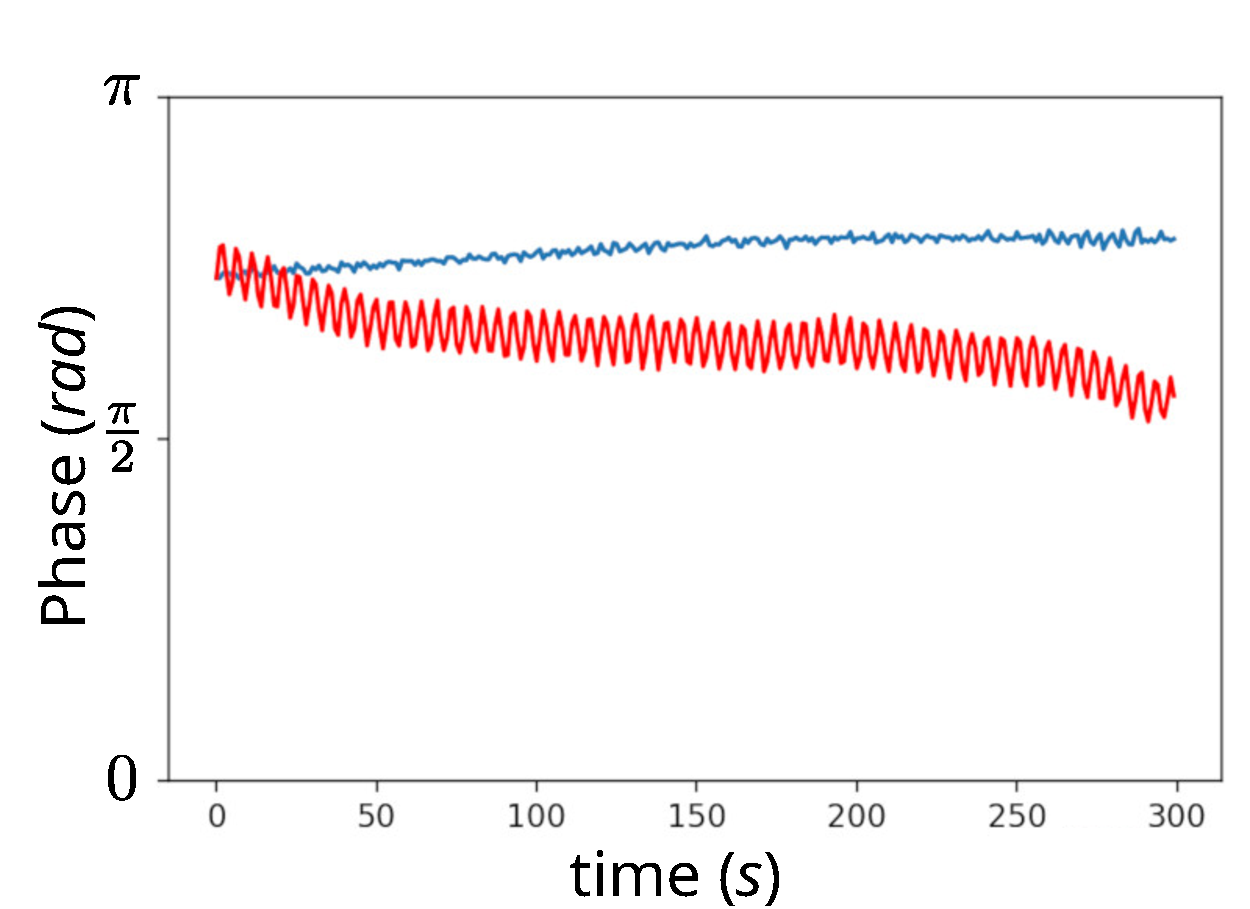
\includegraphics[width = 0.75\textwidth]{images/phase_vibrations.pdf}
  \caption{
    \textbf{Vibration induced phase fluctuations.}
    Phase fluctuations measured over time at
    a specific position on a plane located at the distal end of a multimode fiber.
    We employ off-axis holography using the setup depicted in Fig.~\ref{fig:MMF_ref}.
    The red and blue curves correspond to the phase fluctuations
    measured respectively without and with vibration damping
    by securing the flat cable with foam, as illustrated in Fig.~\ref{fig:dumping}.
  }
  \label{fig:phase_vibrations}
\end{figure}


A simple yet effective solution consists in dampening the vibrations
at the flat cable's level by clamping it with a soft material,
as depicted in Fig.~\ref{fig:dumping}.
This can be achieved using commonly available materials.
In this context, we utilize simple foam, typically used for packaging, and secure it to the cable
with two metallic plates, screws, and nuts.
We observe a significant decrease in the phase fluctuations,
as demonstrated in Fig.~\ref{fig:phase_vibrations} (blue curve).\\



\begin{figure}[ht]
  \centering
  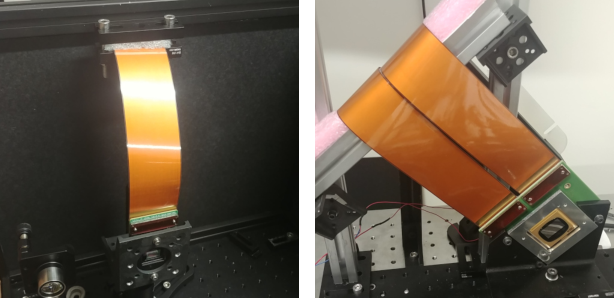
\includegraphics[width = 0.95\textwidth]{images/dumping.pdf}
  \caption{
    \textbf{Dumping mechanical vibrations.}
    Pictures of experimental setups where a damping of the vibrations is implemented.
    (a) The flat cable is secured with foam and metallic plates.
    (b) The flat cable is in tension against a foam material supported by a metallic plate.
  }
  \label{fig:dumping}
\end{figure}

\begin{tldr}
  \textbf{TL;DR:}\\
  The functioning of DMDs can be perturbed by vibrations transmitted from the electronics board
  via the rigid flat cable that links it to the DMD chip.
  This adverse effect can be minimized by securing the cable with a soft material
  that serves to dampen these vibrations.
\end{tldr}

\subsection{Thermal stability}

Electronics utilized to control the DMD chip experience thermal variations during operation.
The dynamics of this effect are dependent on the frame rate.
Specifically, the chips heats up more quickly when increasing the frame rate.
The increase of temperature can reach more than $15$ degrees Celsius
when running a sequence at maximum speed (20-30 kHz)~\cite{Rudolf2021thermal}.
Notably, this effect is less pronounced when the device is on but not running a sequence.
Temperature fluctuations can cause deformations on the chip's surface
and can modify the phase response of the glass protective window.
This creates low order aberrations, which degrade the quality of the wavefront.
While this issue is comparatively less critical than static aberrations and mechanical instabilities
previously detailed,
it nonetheless has a substantial impact on the complex medium's response
when a DMD is employed to modulate the input wavefront.\\



Before initiating a wavefront shaping experiment,
it is important to characterize the influence of temperature
to assess the extent to which it impacts the results.
Although the exact effect on the wavefront distortion can be directly quantified~\cite{Rudolf2021thermal},
it is typically more convenient
to directly measure the effect on the studied system's response.
To do so, we use a setup similar to the one presented in the previous section
and depicted in Fig.~\ref{fig:MMF_ref}.
We can then estimate the field or intensity decorrelation over time.
We present here results with intensity correlation, as it does not require a reference arm.
The measured output pattern typically take the form of a seemingly random speckle pattern,
that is sensitive to minute changes in the input wavefront.
The correlation estimation is obtained by comparing the output intensity pattern
$I(\vec{r}, t)$ at a given time $t$
to the one at $t=0$.
We use the following expression for the correlation:



\begin{equation}
  C(t) =
  \frac{
    \left\langle
    \bar{I}(\vec{r}, t) \bar{I}(\vec{r}, t=0)
    \right\rangle_{\vec{r}}
  }{
    \sqrt{
      \left\langle
      \bar{I}(\vec{r}, t)^2
      \right\rangle_{\vec{r}}
      \left\langle
      \bar{I}(\vec{r}, t=0)^2
      \right\rangle_{\vec{r}}
    }
  } \, ,
  \label{eq:temp_decorr}
\end{equation}




with $\bar{I}(\vec{r}, t) = I(\vec{r}, t) - \left\langle I(\vec{r}, t) \right\rangle_{t}$
and $\left\langle . \right\rangle_{\vec{r}}$.
$\left\langle . \right\rangle_{t}$
represent the spatial averaging over the region of interest
of the output plane (i.e. the plane of the camera sensor)
and the temporal averaging over the measured frames.
Fig.~\ref{fig:temp_decorr} shows the measured decorrelation
over time when running an sequence in an infinite loop.
$t=0$ correspond in the first case (a)
to the start of a sequence
and is set in the second one to
4.2 hours post the after of the sequence (b).
For the scenario (a), it is to note that before the sequence commenced,
the DMD was active but remained in the idle state,
meaning that it was not executing a sequence.
We observe a non-negligible decorrelation over time
after the sequence started
that slows down after about 1 hour.
When running the same experiment 4.2 hours after starting the sequence,
the correlation is now stable.\\



\begin{figure}[ht]
  \centering
  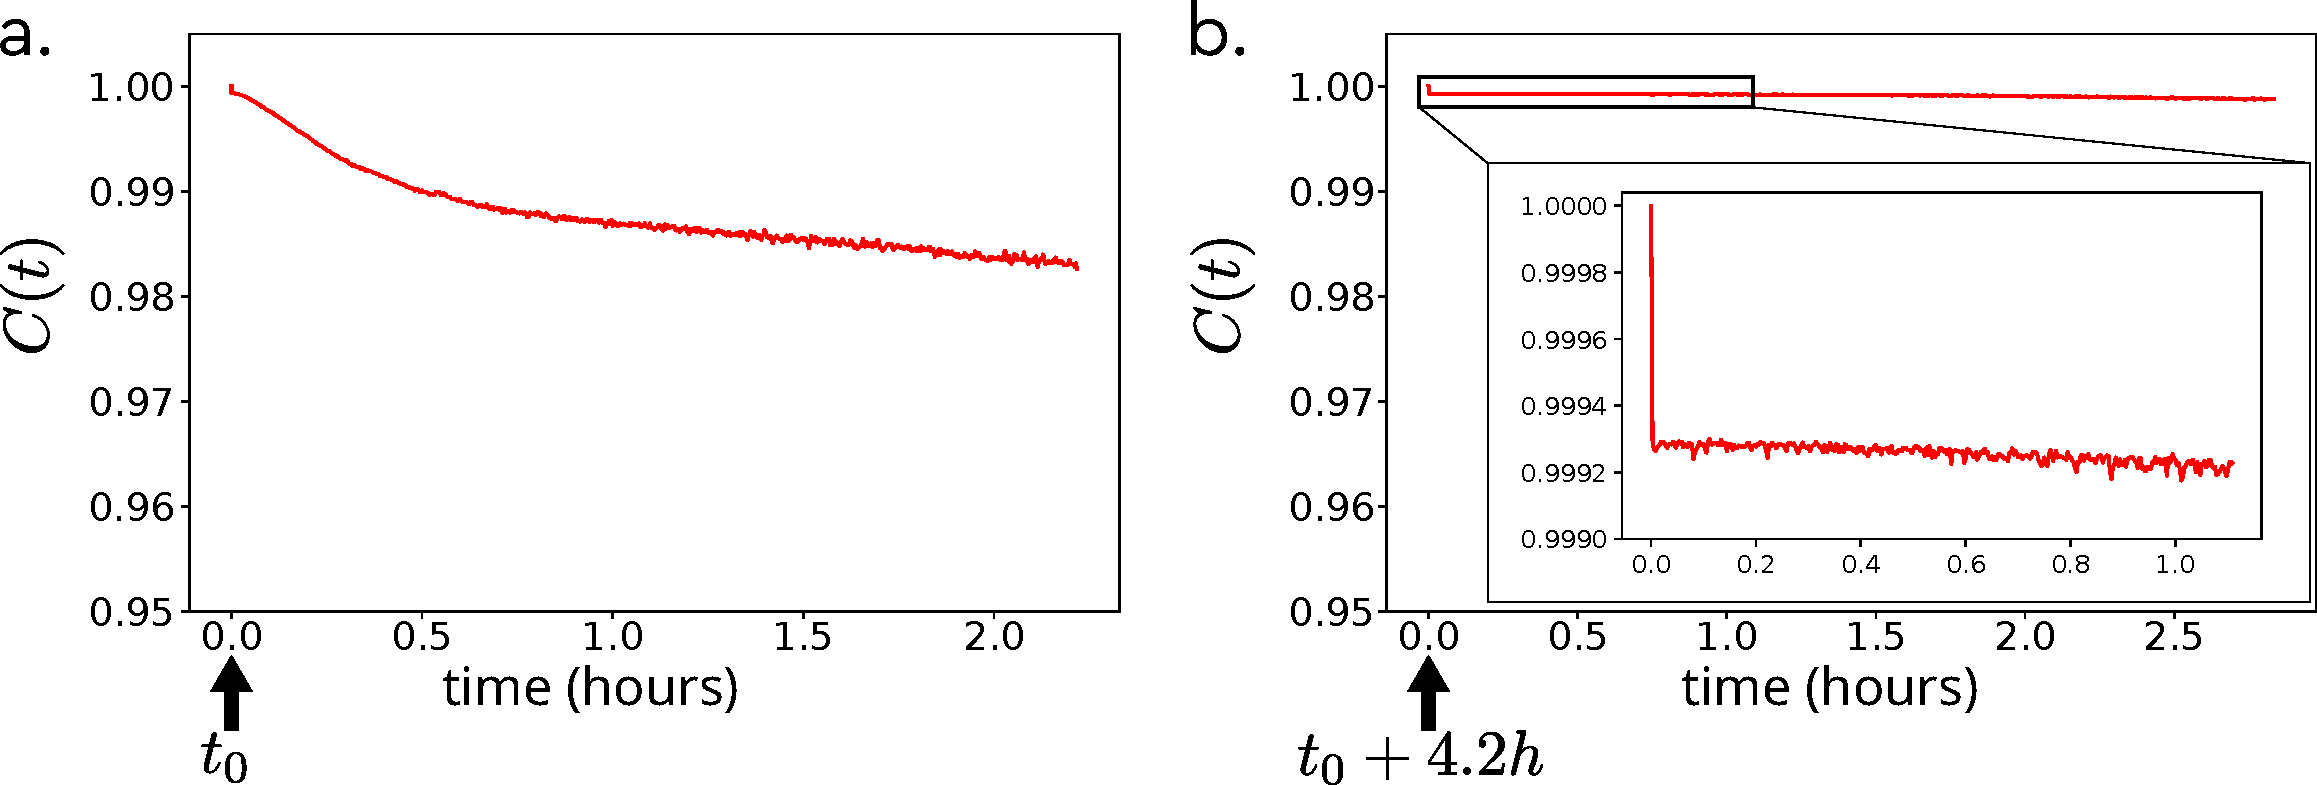
\includegraphics[width = 0.95\textwidth]{images/DMD_decorrelation_T.pdf}
  \caption{
    \textbf{Effect of temperature.}
    Temporal decorrelation of a speckle pattern measured at the output of a multimode fiber
    when running a sequence in an infinite loop.
    We use Eq.(\ref{eq:temp_decorr}) to estimate the correlation between the intensity pattern
    at a given time $t$ and the one at $t=0$.
    $t=0$ corresponds respectively to the start of the sequence (a)
    and to 4.2 hours after the start of the sequence (b).
  }
  \label{fig:temp_decorr}
\end{figure}

The more efficient way to counteract this effect is to use a
closed-loop system to stabilize the temperature of the DMD chip.
This can be achieved by using a thermoelectric cooler
as demonstrated in Ref.~\cite{Rudolf2021thermal}
and depicted in Fig.~\ref{fig:decorr_T}.

\begin{figure}
  \centering
  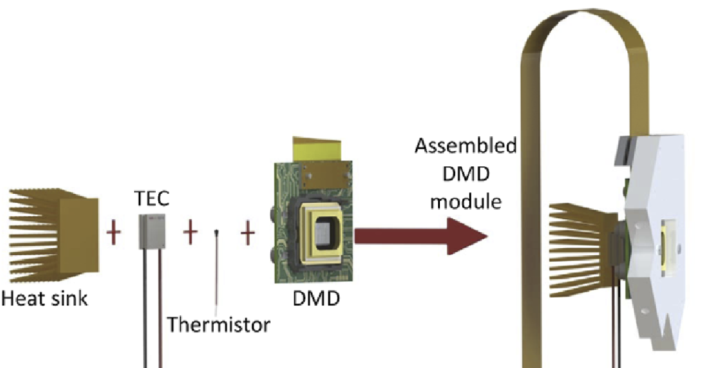
\includegraphics[width = 0.65\textwidth]{images/Cizmar_1.pdf}
  \caption{
    \textbf{Thermal stabilization of the DMD chip.}
    Schematic representation of the setup utilized to regulate the temperature of the DMD chip.
    A thermoelectric cooler and a heat sink is employed to control the temperature,
    while a thermistor is used to measure deviations from the temperature setpoint.
    A closed-loop system is used to regulate the temperature.
    Image adapted from~\cite{Rudolf2021thermal}.
  }
  \label{fig:decorr_T}
\end{figure}

\begin{tldr}
  \textbf{TL;DR:}\\
  DMDs take about an hour to thermaly stabilize when a sequence is running.
  It can countered by using a thermoelectric cooler
  and a temperature sensor.
  It can also be simply mitigated by letting a sequence run for few hours
  before starting the experiment.
\end{tldr}

% \section{Control Vialux DMDs with Python}

% \cite{hofling2004alp}

% \cite{popoff2016alp4lib}

\section{Acknowledgments}
Authors wishing to acknowledge assistance or encouragement from
colleagues, special work by technical staff or financial support from
organizations should do so in an unnumbered `Acknowledgments' section
immediately following the last numbered section of the paper. In \verb"iopart.cls" the
command \verb"\ack" sets the acknowledgments heading as an unnumbered
section.

\section{Bibliography}


\bibliographystyle{unsrt}
\bibliography{biblio}

\end{document}

